% Bug ancrages pdf à cause du bricolage entre PARTIES et chapitres avec l'intro, méthodes et discussion...
% See https://tex.stackexchange.com/questions/71162/reset-section-numbering-between-unnumbered-chapters
\setcounter{section}{0} % 
\renewcommand*{\theHsection}{Methodes.\the\value{section}}

% COVER PAGE
\centerline{\bfseries\textcolor{bleusection}{ \Huge Méthodes}}  

\bigskip

% Figure cover
\begin{tikzpicture}
  \def\ig{%
   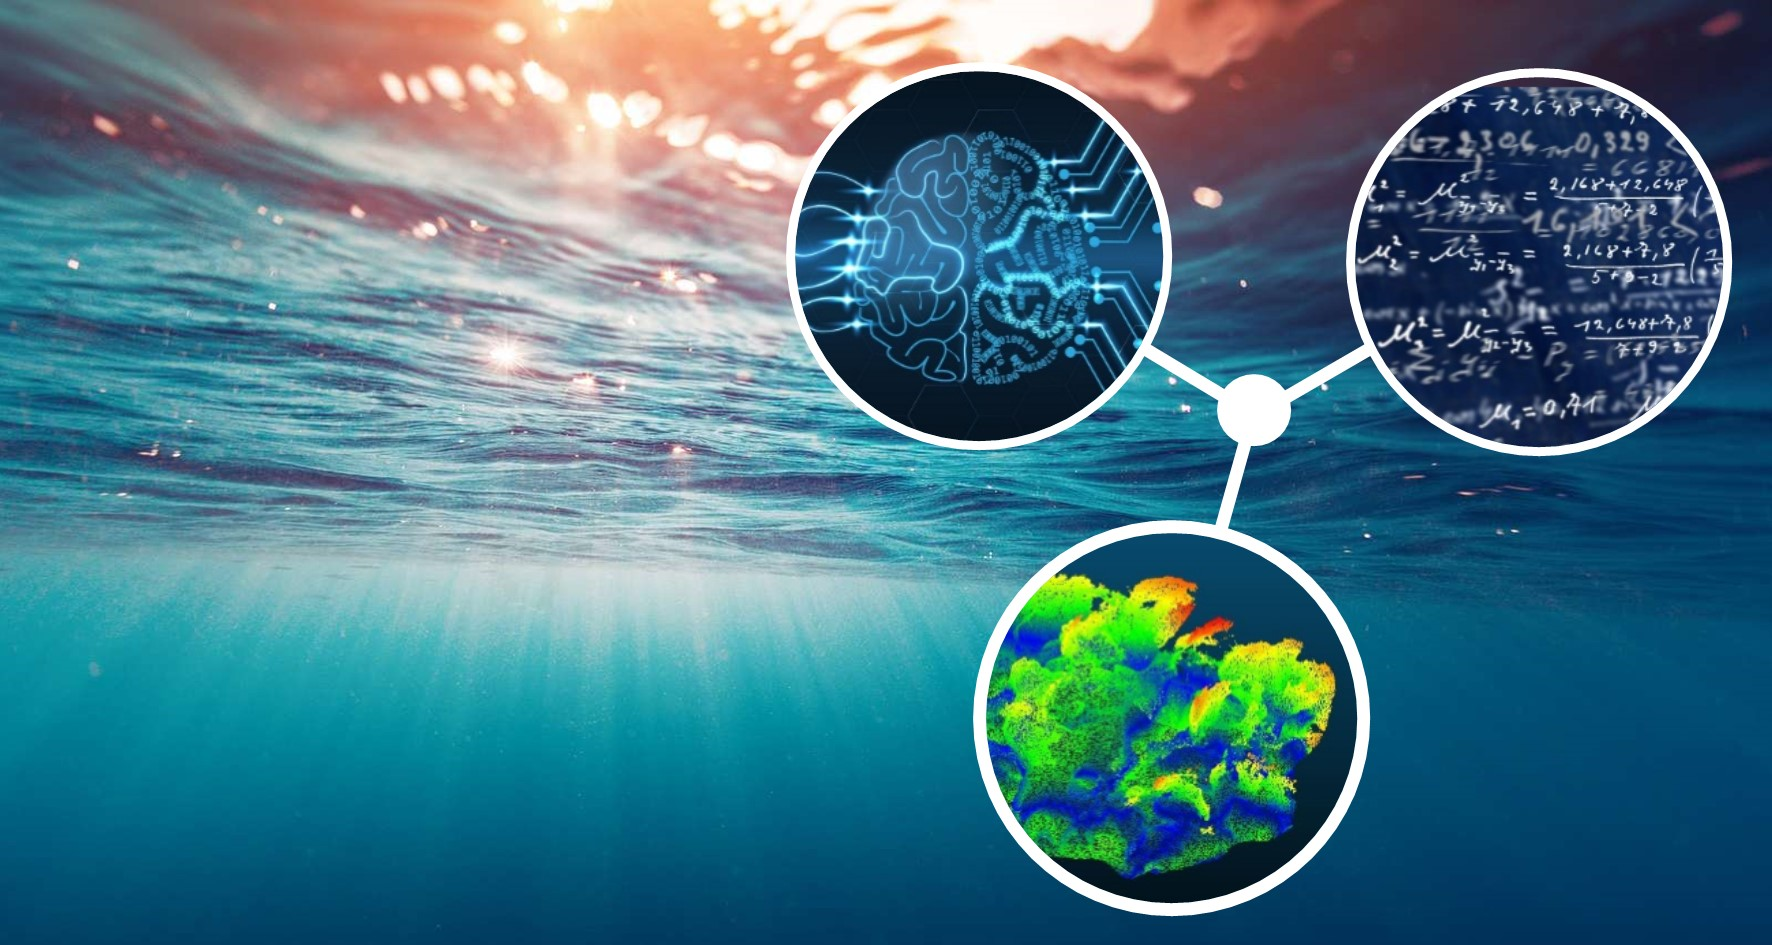
\includegraphics[width=\linewidth,keepaspectratio]{./2_methodes/cover_methodes}}
 \node [inner sep=0pt](mypicture) at (0,0) {\phantom{\ig}};
 \clip[rounded corners=5mm] ($(mypicture.south west)+(\bord,\bord)$) rectangle ($(mypicture.north east)-(\bord,\bord)$);
 \node[inner sep=0pt](mypicture) at (0,0) {\ig};
\end{tikzpicture}

% Table des matières méthodes
{\LARGE
\begin{enumerate}[label=\textcolor{bleusection}{\arabic*}{.}, leftmargin=2cm]
  \item \nameref{methodes.1}
  \item \nameref{methodes.2}
\end{enumerate}
}

% DEBUT METHOGOLOGIE
\clearpage
\pagestyle{methodo}

\section{Analyses d'images par apprentissage profond}\label{methodes.1}

L’analyse d’images est un champ de recherche très actif, qui a pour but d’interpréter automatiquement le contenu d’une image afin d’y détecter un objet (i.e. détection), de segmenter l’image en zones de même nature (i.e. segmentation), de reconnaître des objets (i.e. classification), ou encore de mesurer une variable continue à partir de la structure de l’image (i.e. régression). L’analyse d’images a connu d’importants rebondissements depuis une dizaine d’années, grâce à l’explosion de la puissance de calcul (notamment l’utilisation des cartes graphiques, ou « Graphical Processing Unit » (GPU)) et à l’apparition de nouveaux algorithmes : les Réseaux de Neurones Convolutifs (RNC). Nous détaillerons dans cette section l’utilisation des RNC à des fins de classification d’images.

\subsection{Structure des réseaux de neurones convolutifs}

Comme leur nom le laisse deviner, les RNC sont cousins des réseaux de neurones, ou « perceptron multicouche », imaginés dans les années 1970 et mis au point par David Rumelhart \citep{rumelhart_learning_1986}. Ces algorithmes visent à simuler les mécanismes d’apprentissage des êtres vivants en reproduisant le fonctionnement d’un système nerveux : de nombreuses unités, les « neurones », sont interconnectées et réagissent à un stimulus en émettant un signal qui parcourt le réseau et produit une réaction ou une interprétation \citep{aggarwal_neural_2018}. L’intensité des signaux entre les différents neurones s’adapte à mesure que l’être vivant est confronté à différentes situations ou stimuli, afin de peu à peu améliorer la réaction ou la capacité de jugement : c’est le phénomène d’apprentissage.

Les RNC sont des réseaux à propagation directe (« feedforward ») qui incluent des couches de convolutions permettant de prétraiter l’information avant qu’elle ne soit analysée par le perceptron multicouche. Les convolutions permettent notamment de réduire significativement le nombre de paramètres pour les grandes images, car dans le cas d’un perceptron multicouche avec un neurone associé à chaque pixel dans la couche d’entrée, le nombre de paramètres augmente exponentiellement avec la taille de l’image. Par ailleurs, les RNC permettent de faire ce que l’on appelle un « apprentissage de bout en bout » (pour « end-to-end learning ») : les couches de convolutions apprennent à extraire les variables les plus pertinentes pour la classification, qu’un perceptron multicouche apprend à interpréter pour produire sa classification (\autoref{figure_methodo1}). Ces architectures contiennent souvent un grand nombre de couches à entraîner, c’est pour quoi il est question « d’apprentissage profond » (ou « deep learning »).

L’idée des convolutions est inspirée d’une étude portant sur le fonctionnement du cortex visuel du chat \citep{hubel_receptive_1959}, qui a montré que certaines régions de son champ de vision semblent exciter spécifiquement certains neurones. La première architecture basique inspirée de cette observation est le Neocognitron \citep{fukushima_neocognitron_1988}, généralisée quelques années plus tard par le travail de LeCun et al. (1998) avec le LeNet-5 capable de reconnaître des chiffres écrits à la main en niveaux de gris. Les RNC ont depuis connu un développement important, notamment 

%%%%%%%%%%%%%%%%%%%%%%%%%%%%%%%%%%%%%%%
%%% Figure methodo1: Structure CNNs %%%
%%%%%%%%%%%%%%%%%%%%%%%%%%%%%%%%%%%%%%%
\begin{sidewaysfigure}
%\enlargethispage{.5cm}
\begin{figure}[H]
	\begin{center}
	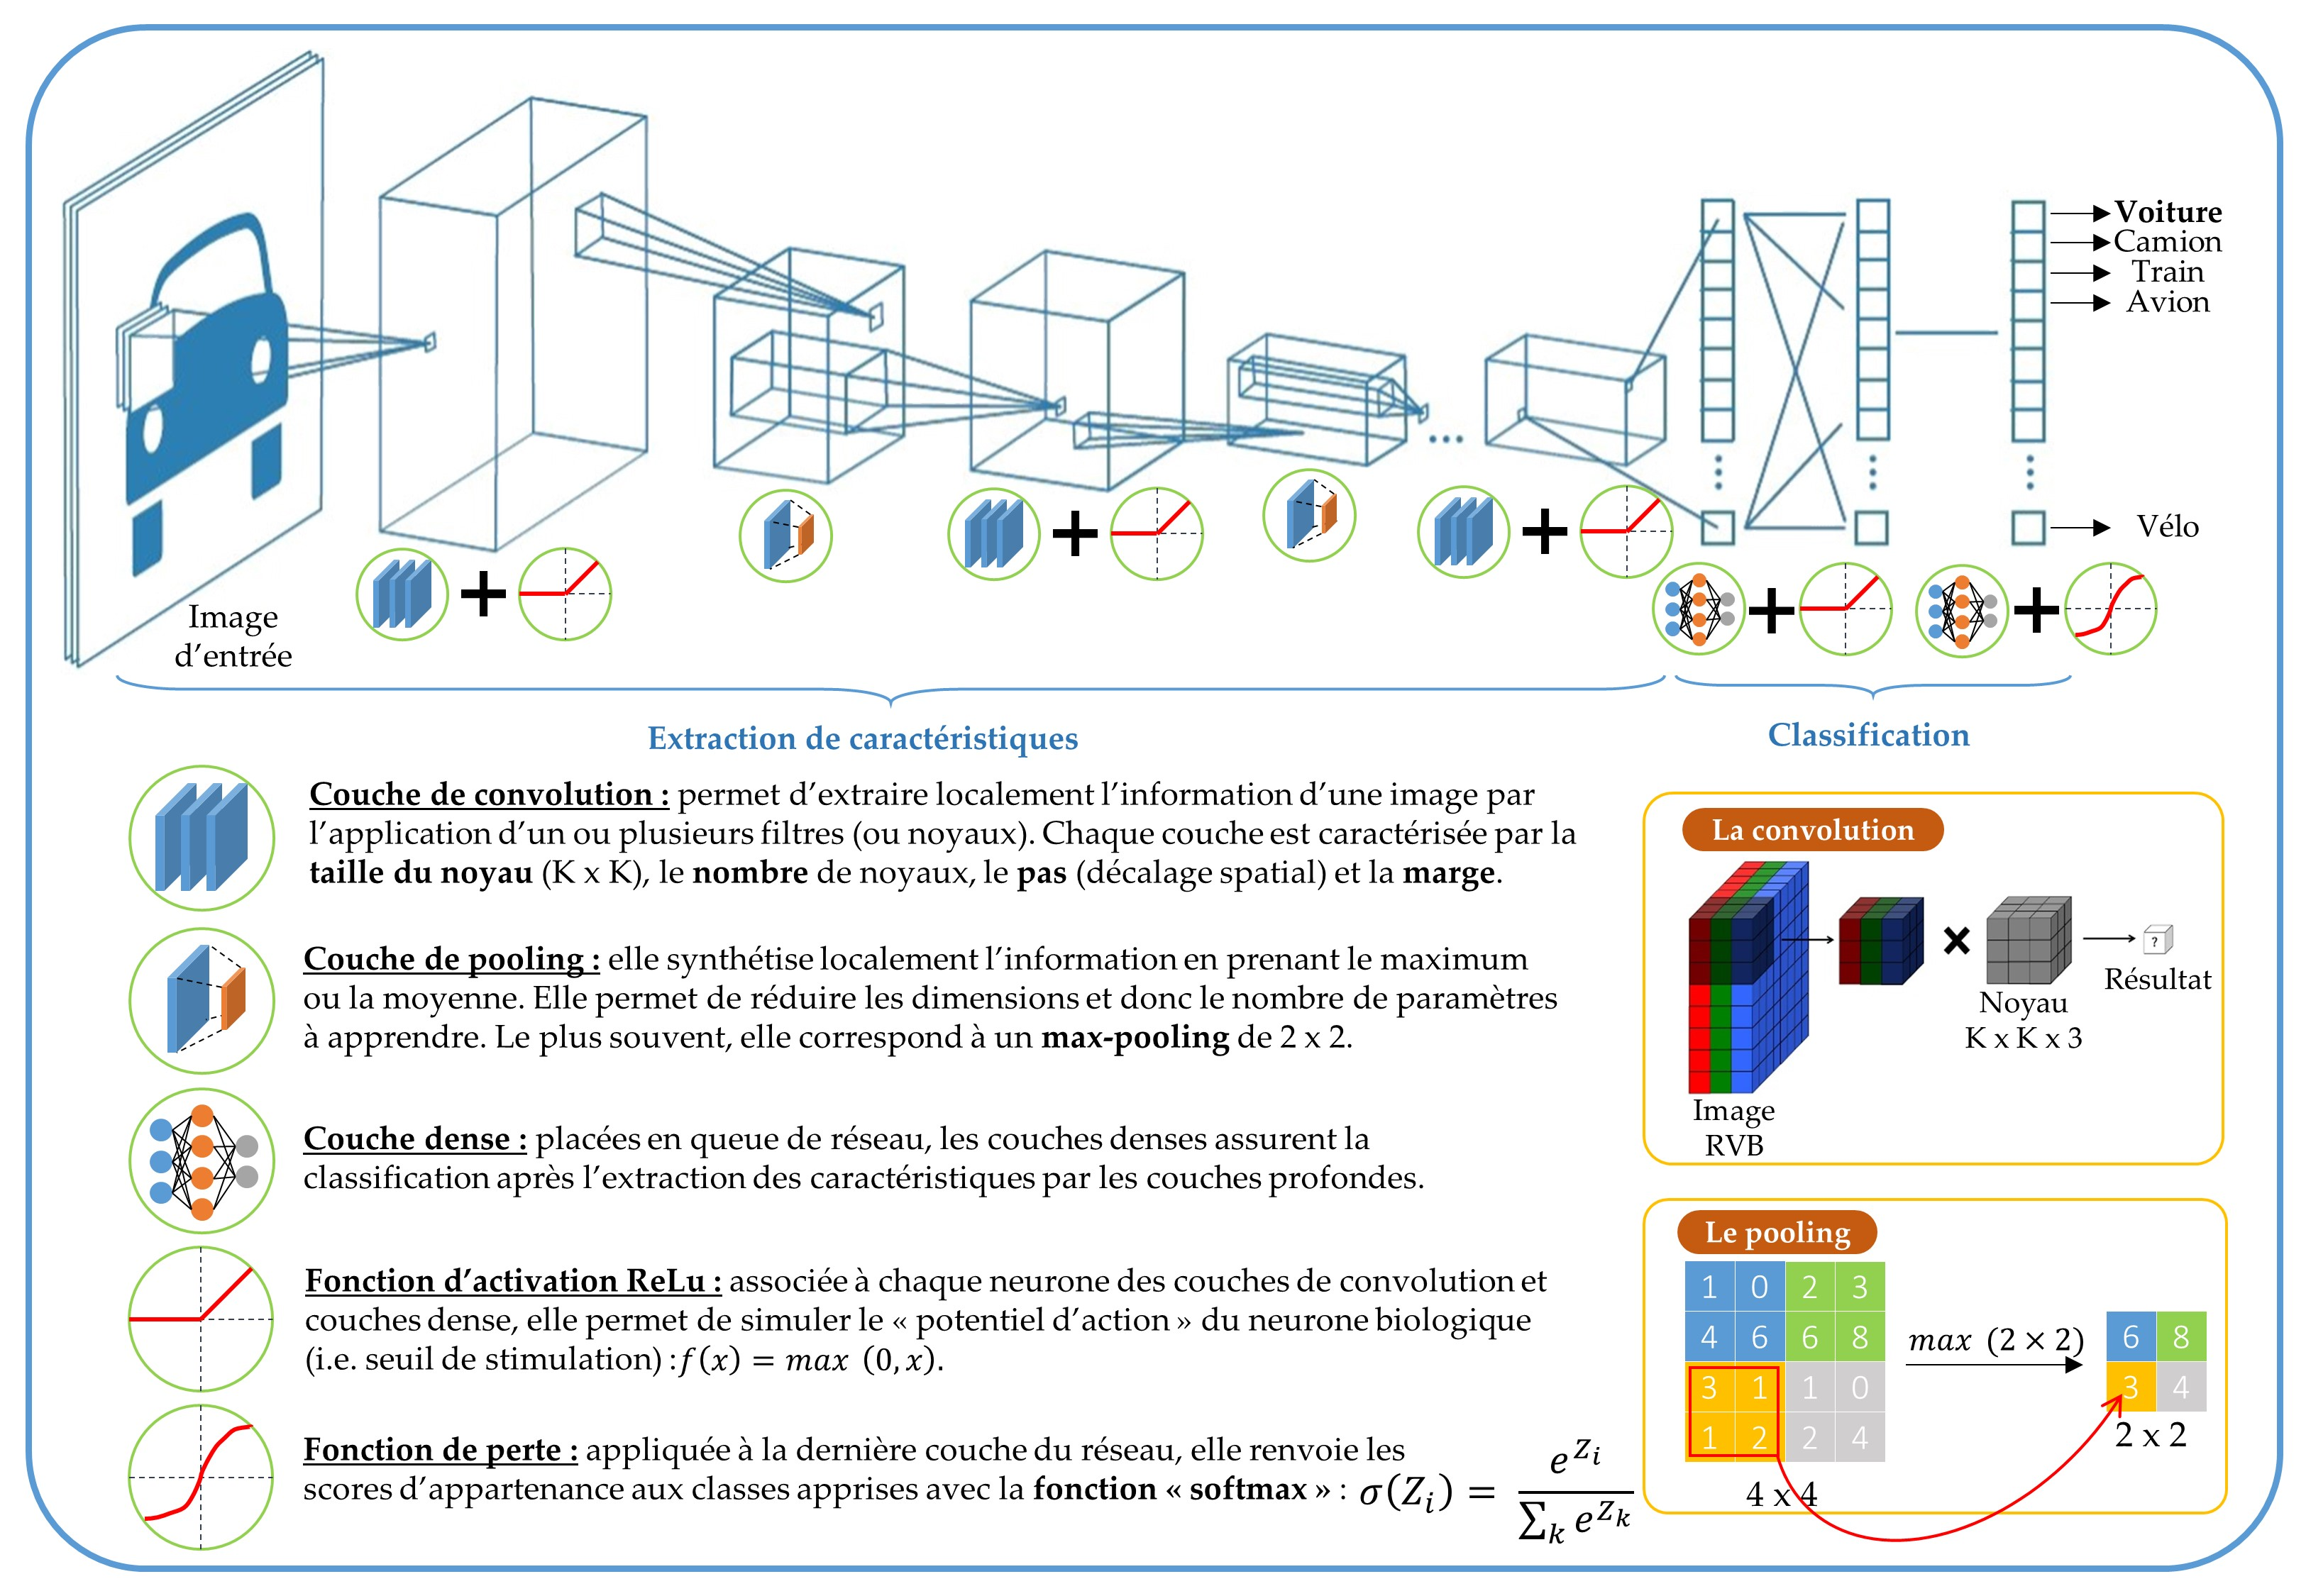
\includegraphics[width=\linewidth,keepaspectratio]{./2_methodes/encart_architecture}
		\caption[Vision schématique de l’architecture d’un réseau de neurones convolutifs destiné à la classification d’images]{Vision schématique de l’architecture d’un réseau de neurones convolutifs destiné à la classification d’images (schéma du réseau adapté de mathworks.com).}
	\label{figure_methodo1}
\end{center}
\end{figure}
\end{sidewaysfigure}

\noindent grâce à l’apparition de grosses bases de données annotées telles qu’ImageNet \citep{deng_imagenet:_2009} et l’augmentation de la puissance de calcul par l’utilisation des cartes graphiques. S’il existe aujourd’hui de nombreuses architectures, chacune ayant apporté sa pierre à l’édifice à un moment donné, les briques élémentaires des RNC sont toujours les mêmes : les couches de convolution, les couches de pooling et les couches denses \citep{lecun_deep_2015} (\autoref{figure_methodo1}).

\subsubsection{Les couches de convolution}

Une convolution permet d’extraire localement l’information d’une image à l’aide d’un filtre mobile, appelé « noyau de convolution », et produire une nouvelle image. Chaque pixel de l’image produite correspond à la combinaison linéaire des valeurs des pixels voisins de l’image d’entrée, dont les coefficients (« poids ») correspondent aux valeurs définies dans le noyau. Pour bien comprendre ce concept, il est important de souligner qu’une image peut posséder plusieurs canaux de couleurs, et donc elle doit être vue comme un volume (hauteur × largeur × canaux de couleurs). Par exemple, une image Rouge-Vert-Bleu (RVB) de 32 $\times$ 32 pixels sera représentée par un volume de 32 $\times$ 32 $\times$ 3, chaque tranche correspondant à un canal de couleur. Une convolution correspond dans ce cas à l’application d’un noyau à trois dimensions, glissant sur toute la hauteur et la largeur de l’image, en incluant tous les canaux de l’image (voir encart « La convolution », \autoref{figure_methodo1}), pour produire une image à deux dimensions (profondeur de 1). Dans le cas d’une image en dégradé de gris, à un seul canal, le noyau est donc de dimensions largeur $\times$ hauteur $\times$ 1. Le noyau est invariant en fonction des dimensions spatiales de l’image, i.e. les poids sont constants tandis que le noyau glisse sur l’ensemble de l’image. Cette propriété rend une convolution indépendante d’une translation de la donnée d’entrée. Généralement, une couche de convolution est constituée de plusieurs noyaux afin d’extraire différentes informations de l’image d’entrée.

Les quatre hyperparamètres d’une couche de convolution sont :

\begin{itemize}
    \item \textbf{La taille du noyau (« kernel size ») :} largeur $\times$ hauteur du filtre, en pixels (la profondeur est toujours égale au nombre de canaux de l’image en entrée). La taille du noyau définit le niveau d’information extraite : plus elle est petite, plus le noyau extrait une information locale~;
    
    \item \textbf{Le nombre de filtres :} nombre de noyaux utilisés dans la couche. Les poids de chaque noyau sont appris par le réseau afin d’extraire les prédicteurs les plus pertinents au vu de la tâche de classification. Le nombre de noyaux permet de contrôler le volume de sortie et de gérer la dimensionnalité dans le réseau ;
    
    \item \textbf{Le pas (« stride ») :} décalage spatial entre deux applications du noyau sur l’image, en pixels. Un pas de un fera glisser le noyau d’un pixel par un pixel sur l’image en entrée, et produira ainsi une image en sortie de même dimension spatiale. Plus le pas est grand, plus la dimension spatiale de l’image de sortie sera petite ;
    
    \item \textbf{La marge (« padding ») :} l’application du noyau pose un problème lorsque l’on se trouve sur les bordures de l’image, où il est impossible de réaliser les calculs pour ces pixels. Sans ajout d’une marge à l’image d’entrée, la convolution produit donc une image de plus petites dimensions spatiales. Afin de conserver les dimensions, il est courant d’ajouter une marge à l’image d’entrée (de largeur ($K$ – 1) / 2 si $K$ est la largeur du noyau), généralement remplie de zéros \citep{aggarwal_neural_2018}.
    
\end{itemize}

\subsubsection{Les couches de pooling}

L’opération de « pooling » (ou « mise en commun ») (voir encart « Le pooling », \autoref{figure_methodo1}) est utilisée pour réduire la dimension des couches de convolution, elle est généralement placée entre des blocs de convolutions. Elle permet de réduire le nombre de paramètres à apprendre, et donc diminue les temps de calcul et permet d’éviter le phénomène de surapprentissage (« overfitting »). La couche de pooling opère indépendamment sur chaque partie du bloc de convolution en entrée (sur toute sa profondeur, il s’agit donc d’un volume) qu’elle réduit en utilisant une fenêtre mobile, ce qui augmente l’invariance du réseau à de petites transformations géométriques. Elle ne possède que deux hyperparamètres : la \textbf{taille} de la fenêtre et le \textbf{pas} (la fonction est déterminée, généralement la moyenne ou le maximum). La plupart du temps, la couche de pooling calcule la valeur maximale et utilise un pas et une taille de fenêtre égaux à 2. 

\subsubsection{Les couches denses}

Après l’extraction des prédicteurs par les couches de convolution et de pooling, la classification est assurée par un perceptron multicouche qui prend en entrée le résultat de la dernière couche de convolution, et produit en sortie le résultat de la classification. Ce perceptron multicouche est composé de plusieurs « couches denses » (ou « couches entièrement connectées ») : une « couche d’entrée », une ou plusieurs « couches cachées » et une « couche de perte » (c’est elle qui produit le vecteur de scores d’appartenance aux différentes classes). Dans une couche dense, les neurones artificiels ont des connexions avec toutes les sorties de la couche précédente (\autoref{figure_methodo2}).

%%%%%%%%%%%%%%%%%%%%%%%%%%%%%%%%%%%%%%%%%%%
%%% Figure methodo2: Les couches denses %%%
%%%%%%%%%%%%%%%%%%%%%%%%%%%%%%%%%%%%%%%%%%%
\begin{figure}[H]
	\begin{center}
	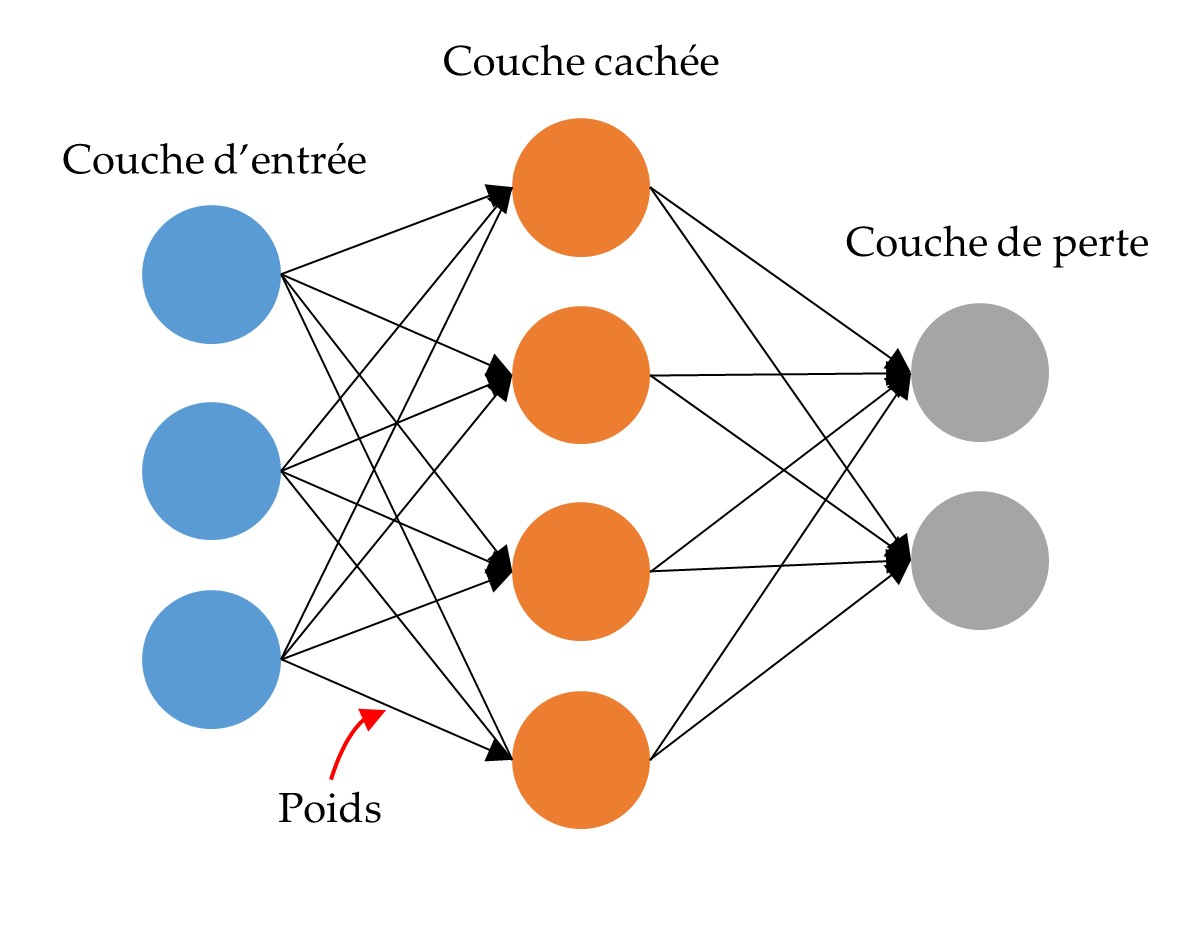
\includegraphics[width=0.7\linewidth,keepaspectratio]{./2_methodes/MLP}
		\caption[Fonctionnement schématique d’un perceptron multicouche en sortie d’un réseau de neurones convolutifs]{Fonctionnement schématique d’un perceptron multicouche en sortie d’un réseau de neurones convolutifs.}
	\label{figure_methodo2}
\end{center}
\end{figure}

Les neurones d’une couche dense en position N réalisent une combinaison linéaire des valeurs émises par les neurones de la couche $N-1$, avec un poids unique par connexion. Si la couche $N$ contient $P_N$ neurones et la couche $N-1$, $P_{N-1}$ neurones, le nombre de poids associés à la couche $N$ (liens entre les couches $N-1$ et $N$) est : $P_N$ $\times$ $P_{N-1}$.

\subsubsection{Les fonctions d'activation}

A chaque combinaison linéaire réalisée par les couches de convolution et couches denses est appliquée une fonction d’activation. Cette fonction permet de simuler le comportement d’un neurone biologique et son « potentiel d’action » (i.e. seuil de stimulation), afin d’améliorer l’efficacité du traitement de l’information. Il existe de nombreuses fonctions d’activation, mais depuis le développement du réseau AlexNet \citep{krizhevsky_imagenet_2012}, la fonction la plus répandue est la fonction ReLu (pour « Rectified Linear unit »), définie par l’équation suivante :

\begin{equation}
    f(x)=\max{(0,x)}
    \label{eqmethodes.1}
\end{equation}

La fonction ReLu introduit de la non-linéarité dans le réseau, ce qui permet d’accélérer \\l’apprentissage sans significativement impacter les performances \citep{krizhevsky_imagenet_2012}.

La dernière couche du réseau, appelée « couche de perte », spécifie comment l’entraînement du réseau pénalise l’écart entre le signal prévu et le signal réel. Dans le cas d’une classification où le résultat attendu est la prédiction d’une classe unique, elle produit un vecteur de scores d’appartenance aux différentes classes et elle se différencie des couches denses de deux manières : (i) sa taille est égale au nombre de classes considérées, et (ii) la fonction d’activation de cette couche est la fonction « softmax » définie comme suit :

\begin{equation}
\sigma(z_i) = \displaystyle\frac{e^{z_i}}{\displaystyle\sum_{k} e^{z_k}}\ avec \ i = 1,...,n
\end{equation}

Avec $Z = {Z_1, Z_2, ..., Z_n}$ les valeurs issues de chaque neurone de la dernière couche, appelés « logits ». Cette fonction d’activation contraint le vecteur en sortie à prendre des valeurs entre 0 et 1 et dont la somme est égale à 1. De ce fait, les scores obtenus peuvent être considérés comme des probabilités que l’image en entrée appartienne à chaque classe considérée, représentés par la position de chaque valeur au sein du vecteur de scores (et permettent de mesurer l’erreur commise par le réseau lors de l’entraînement, avec une fonction de coût). Généralement, la prédiction finale est faite en prenant le score maximal $max(\sigma(z))$, ce que l’on appelle « Softmax Response » (SR).

\medskip

\setlength{\fboxsep}{5pt}
\setlength{\fboxrule}{0.6pt}
\noindent\framebox{%
  \begin{minipage}{\linewidth}
    Les RNC sont de puissants algorithmes d’\textbf{analyse d’images}. Ils sont structurés en \textbf{couches} de différentes natures (convolutions, pooling, denses) qui utilisent des \textbf{fonctions d’activation} permettant d’améliorer l’efficacité du traitement. Les premières séries de couches assurent l’\textbf{extraction} et la \textbf{synthèse des caractéristiques} de l’image, que les couches finales \textbf{interprètent} pour \textbf{classifier le contenu} de l’image.
  \end{minipage}
}

\subsection{Une diversité d'architectures}

Avant l’apparition des RNC, tout apprentissage automatique réalisé sur des images se basait sur l’extraction préalable de prédicteurs calculés par des filtres construits « à la main » \citep{kumar_detailed_2014}. Cette tâche, appelée « feature engineering », nécessitait généralement de calculer un grand nombre de filtres puis de sélectionner ceux apportant le plus d’informations pour la tâche souhaitée (par des méthodes de sélection de variables). Les RNC ont révolutionné cette approche en incluant la construction des filtres dans le processus d’apprentissage automatique, permettant d’automatiser l’extraction des caractéristiques de l’image et sa classification, ce que l’on désigne par « apprentissage de bout en bout ».

Les RNC ont marqué l’histoire de l’apprentissage supervisé en 2012 avec le réseau AlexNet, composé de huit couches et 60 millions de paramètres \citep{krizhevsky_imagenet_2012}, qui a gagné 10 \% de précision par rapport au meilleur algorithme sur le concours de classification d’images ImageNet \citep{deng_imagenet:_2009}. Depuis, les RNC se sont approfondis et ont gagné en performance avec le développement de nombreuses architectures : VGGNet \citep{simonyan_very_2015}, GoogLeNet \citep{szegedy_going_2015}, ResNet \citep{he_deep_2016}, DenseNet \citep{huang_densely_2017}… (\autoref{figure_methodo3}). Il semblerait que la reconnaissance d’images avec ces algorithmes ait aujourd’hui atteint son potentiel maximum \citep{rawat_deep_2017}, avec les performances hors du commun des RNC sur des jeux de données tels qu’ImageNet. 

%%%%%%%%%%%%%%%%%%%%%%%%%%%%%%%%%%%%%%%%%%%%%%%%%%%%%%
%%% Figure methodo3: Les principales architectures %%%
%%%%%%%%%%%%%%%%%%%%%%%%%%%%%%%%%%%%%%%%%%%%%%%%%%%%%%
\begin{figure}[H]
	\begin{center}
	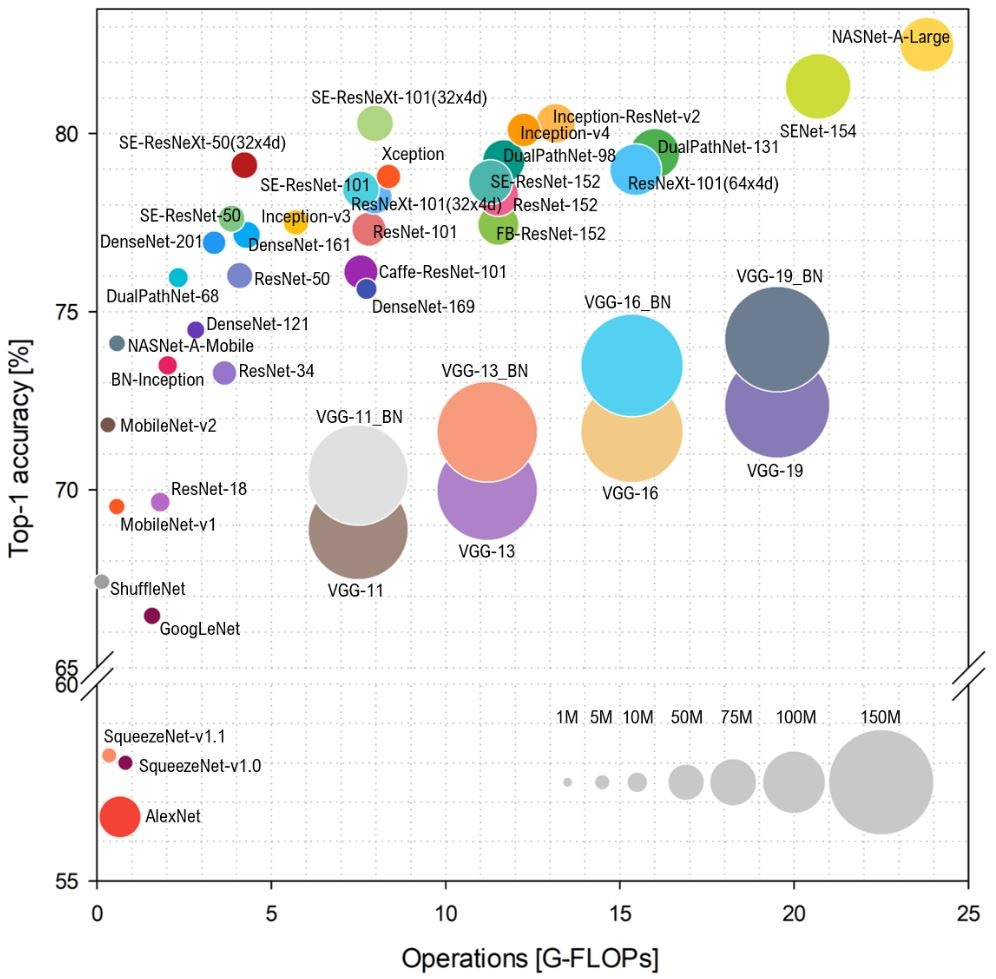
\includegraphics[width=0.7\linewidth,keepaspectratio]{./2_methodes/benchmark_deepLearning_Bianco2018}
		\caption[Graphique représentant la performance (« top-1 accuracy ») des grandes architectures sur le jeu de données ImageNet]{Graphique représentant la performance (« top-1 accuracy ») des grandes architectures sur le jeu de données ImageNet en fonction de la complexité de sa mise en œuvre  G-FLOPS = Giga FLoating-point Operations: nombre d’opérations numériques pour réaliser une inférence; la taille des disques correspond aux millions de paramètres à apprendre \citep{bianco_benchmark_2018}.}
	\label{figure_methodo3}
\end{center}
\end{figure}

\subsection{Stratégies d'entraînement des réseaux}

Tous les cas d’application et les jeux de données associés ont leurs propres spécificités, et s’il n’est pas possible de donner de recette magique, certaines bonnes pratiques permettent de maximiser les performances des réseaux entraînés \citep{he_bag_2019}. Par ailleurs, l’entraînement des réseaux est généralement coûteux en temps de calcul, et il existe une infinité de paramétrisations possibles, c’est pourquoi il convient d’adopter ces bonnes pratiques afin de converger au plus vite vers la paramétrisation optimale permettant de maximiser les performances du réseau.

\subsubsection{Déroulement de l'apprentissage}

L’apprentissage d’un RNC est un processus itératif au cours duquel les nombreux paramètres du modèle (l’architecture est déterminée au préalable), initialisés au hasard, sont ajustés par des méthodes numériques afin d’obtenir les meilleures performances prédictives. A chaque itération, un lot d’images (« batch ») choisies aléatoirement dans la base de données d’entraînement est fourni au réseau. Celui-ci va prédire une classe ou un score pour chaque image, et une fonction de coût (« loss function ») permettant de quantifier l’erreur du réseau dans sa prédiction pour le lot considéré. L’erreur est rétropropagée à travers tout le réseau afin de réajuster les poids des neurones, de sorte à améliorer la prédiction du réseau (i.e. diminuer la valeur de la fonction de coût), avec ce que l’on appelle une Descente de Gradient Stochastique (DGS ; « Stochastic Gradient Descent »). Lot par lot, tout le jeu de données d’entraînement est ainsi fourni au réseau et à chaque lot, les poids sont réajustés. Ceci correspond à ce que l’on appelle une « époque » (« epoch »), il en faut un certain nombre avant que le réseau n’atteigne ses meilleures performances et termine son apprentissage (\autoref{figure_methodo4}). A chaque époque, les cartes sont redistribuées, et les lots à nouveau formés aléatoirement depuis la base de données d’entraînement. Ainsi, chaque image sera vue par le réseau autant de fois que d’époques. L’apprentissage est considéré comme terminé lorsque, après un certain nombre d’époques, les performances du réseau cessent de croître.

\subsubsection{Le phénomène de surapprentissage (« over-fitting »)}

En machine learning, on parle de surapprentissage (« over-fitting ») lorsqu’un modèle prédictif obtient de meilleures performances sur le jeu de données d’entraînement (« training set ») que sur un jeu de données de validation (« validation set ») que le modèle n’a pas encore « vu » (voir haut de la \autoref{figure_methodo4}). Le modèle peut ainsi s’adapter si bien aux données d’entraînement qu’il en perd sa capacité de « généralisation », i.e. à s’appliquer avec des performances similaires sur un autre jeu de données de même nature. Du point de vue du compromis biais / variance, le phénomène de surapprentissage correspond à un modèle capable de s’adapter à tout jeu de données d’entraînement (faible biais), mais dont les paramètres devraient être fortement modifiés pour s’adapter à un autre jeu de données (forte variance). Cela est d’autant plus probable que le modèle est complexe, avec de nombreux paramètres, c’est pourquoi les RNC sont particulièrement sujets au surapprentissage \citep{li_gradient_2019}. On entend par « régularisation » l’ensemble des techniques permettant d’améliorer les capacités de généralisation d’un algorithme, i.e. diminuer son erreur sur le jeu de validation. Cette amélioration peut être réalisée au détriment de l’erreur d’entraînement.

Pour détecter le surapprentissage et mesurer la capacité d’un RNC à généraliser, il convient de séparer le jeu de données en trois lots : un jeu d’apprentissage (« training set »), un jeu de données de validation (« validation set ») et un jeu de données test (« test set ») :

\begin{itemize}
    \item \textbf{Jeu d’entraînement :} il correspond aux images données en entrée du réseau et qui permettent de réajuster les poids des neurones à chaque itération lors de l’apprentissage~;
    
    \item \textbf{Jeu de validation :} à chaque fois que les poids sont réajustés, le réseau mesure les performances sur ce jeu de données. Ce sont ces performances que l’on suit lors de l’apprentissage et qui permettent d’arrêter l’apprentissage avant de surapprendre le jeu d’entraînement~;
    
    \item \textbf{Jeu de test :} une fois l’apprentissage terminé, on mesure les performances du réseau sur ce jeu de données, entièrement nouveau pour lui et qui permet de mesurer les performances réelles du réseau et sa capacité à généraliser.
\end{itemize}

%%%%%%%%%%%%%%%%%%%%%%%%%%%%%%%%%%%%%%%%%%
%%% Figure methodo4: Entraînement CNNs %%%
%%%%%%%%%%%%%%%%%%%%%%%%%%%%%%%%%%%%%%%%%%
\begin{sidewaysfigure}
%\enlargethispage{.5cm}
\begin{figure}[H]
	\begin{center}
	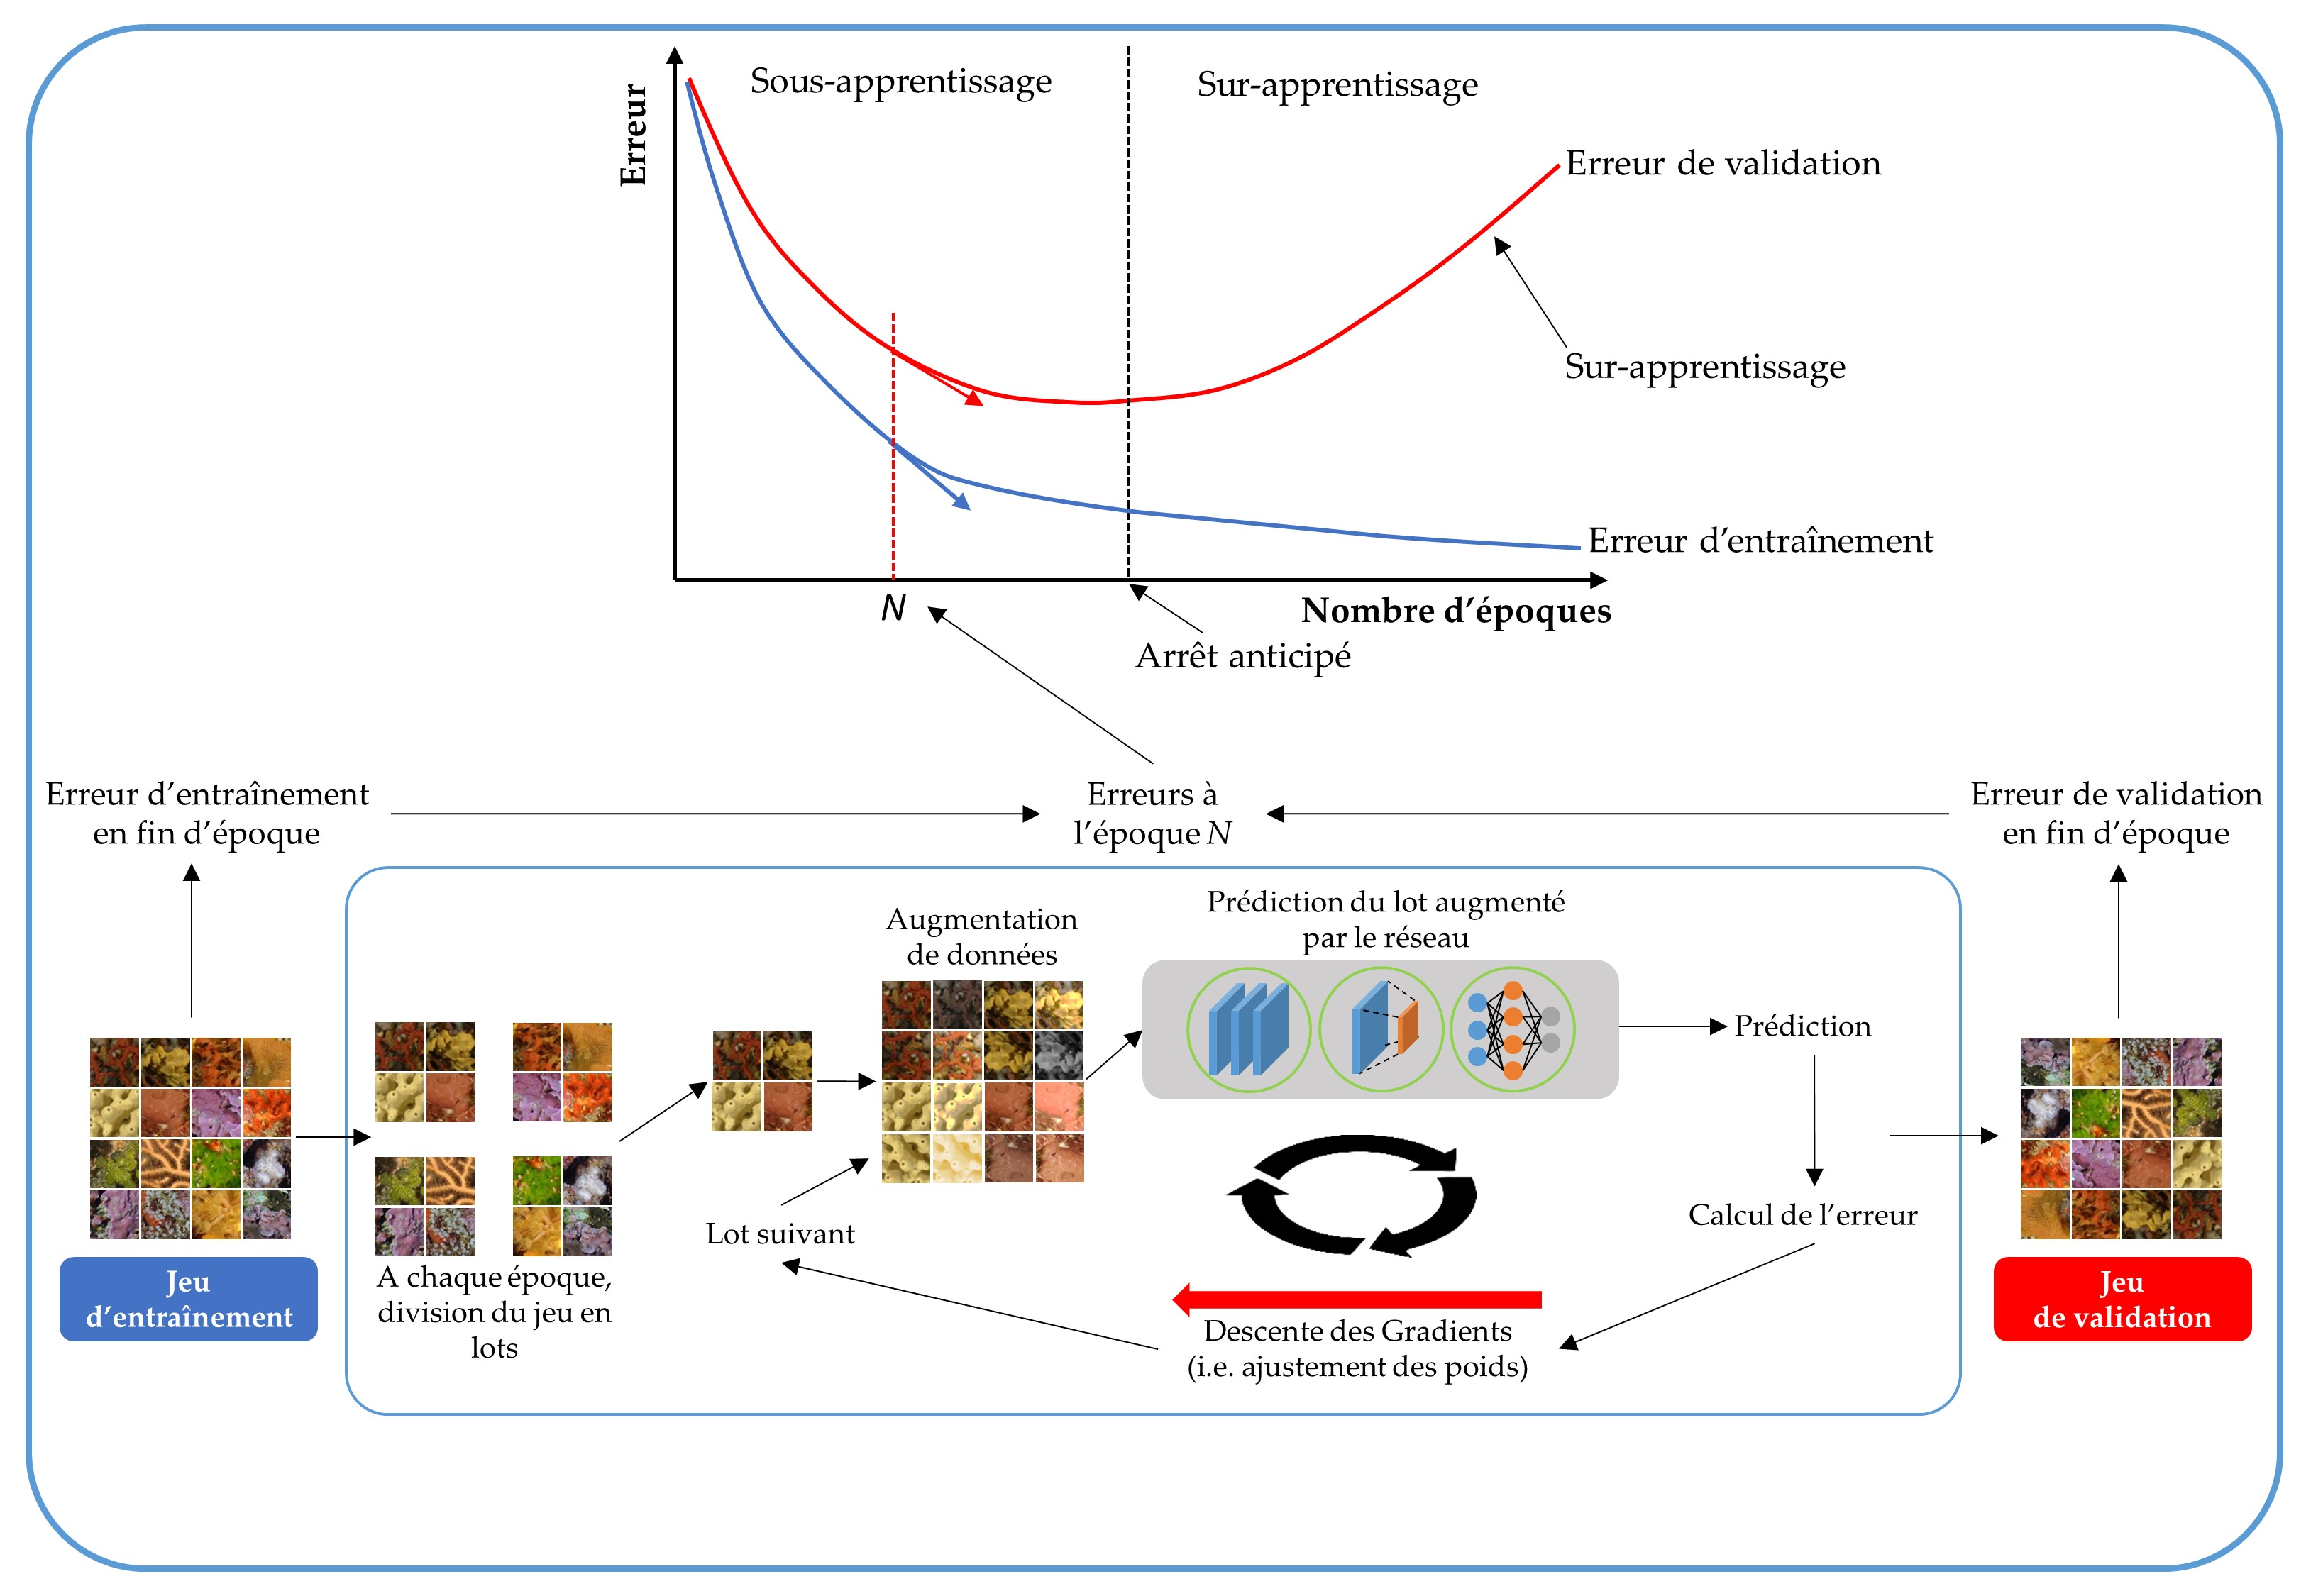
\includegraphics[width=\linewidth,keepaspectratio]{./2_methodes/encart_entrainement}
		\caption[Vision schématique de l’entraînement d’un réseau de neurones convolutifs à reconnaître une image]{Vision schématique de l’entraînement d’un réseau de neurones convolutifs à reconnaître une image.}
	\label{figure_methodo4}
\end{center}
\end{figure}
\end{sidewaysfigure}

La séparation en trois jeux de données dépend de la quantité de données, du nombre de classes et de la difficulté de la tâche à apprendre, mais il est préférable d’utiliser au moins la moitié du jeu de données pour l’entraînement, à condition que les données restantes soient suffisantes pour constituer des jeux de validation et de test représentatifs des variabilités inter et intra-classes.

\subsubsection{Choix de l’architecture et transfert de poids}

Comme vu précédemment, il existe de nombreuses architectures, plus ou moins performantes sur le jeu de données ImageNet, qui correspondent à différentes avancées techniques au fil des années (\autoref{figure_methodo3}). Cependant, le choix de l’architecture ne se dirigera pas nécessairement vers l’architecture ayant les meilleures performances sur le jeu de données ImageNet. En effet, les performances de classification dépendent globalement du nombre de paramètres du modèle, or plus ce nombre augmente plus la quantité de données requises et le temps d’entraînement augmentent. Par ailleurs, plus le rapport nombre de paramètres / quantité de données est élevé, plus le surapprentissage devient problématique. Le choix de l’architecture dépend donc de la quantité de données et de la complexité de la tâche de classification à réaliser. Pour autant, certaines architectures sont aujourd’hui dépassées et ne sont généralement plus utilisées ; c’est le cas d’AlexNet qui a les moins bonnes performances (relativement aux autres architectures de RNC), pour un nombre de paramètres assez important, ou encore VGGNet qui a des performances aujourd’hui considérées comme moyennes pour un nombre très élevé de paramètres.

Dans le cas d’un entraînement à partir de zéro (« from scratch »), l’ensemble des paramètres (i.e. poids) du modèle sont fixés aléatoirement, et leur valeur est ajustée par la DGS à chaque itération jusqu’à convergence. Cependant, il est possible pour les architectures connues d’initialiser les poids avec les valeurs ayant permis de maximiser les performances sur la base de données ImageNet (i.e. transfert de poids ou « transfer learning ») et réaliser l’entraînement pour la tâche souhaitée en ajustant tout ou partie des poids à partir de ces valeurs (i.e. ajustement ou « fine-tuning »). En effet, les premières couches sont relativement peu spécifiques et facilement transférables d’une tâche à l’autre \citep{yosinski_how_2014}. Cette technique a fait ses preuves \citep{huh_what_2016} et elle est couramment utilisée, notamment dans le cas de jeux de données de petite taille \citep{ng_deep_2015}. Il a été montré que les résultats sont d’autant meilleurs que la tâche de classification est proche de la tâche d’origine, mais qu’ils peuvent surpasser les performances atteintes par initialisation aléatoire y compris dans le cas de tâches plus éloignées \citep{yosinski_how_2014}. Par ailleurs, le transfert de poids pourrait augmenter les capacités de généralisation d’un réseau, y compris après l’ajustement des poids \citep{yosinski_how_2014}.

Enfin, comme en apprentissage classique, l’utilisation d’ensembles de réseaux permet parfois d’augmenter les performances prédictives tout en conservant la capacité de généralisation \citep{mehdipour_ghazi_open-set_2016, perez_solo_2019}. Les réseaux composant l’ensemble sont généralement entraînés séparément, puis la décision finale est déterminée par combinaison des prédictions : souvent en prenant la moyenne des prédictions, ou bien en entraînant un perceptron multicouche sur les descripteurs extraits par chacun des réseaux \citep{rokach_ensemble-based_2010}.

\subsubsection{Augmentation de données}

La méthode la plus simple et commune pour régulariser l’apprentissage est ce qu’on appelle « l’augmentation de données » (« data augmentation ») : des images sont générées à la volée à partir des exemples de la base de données d’entraînement, en appliquant des transformations simples telles que des translations, zooms, rotations et miroir / reflet \citep{aggarwal_neural_2018}. En effet, dans la majorité des cas, ces transformations n’affectent en rien les propriétés de l’image et son contenu, ce qui permet d’augmenter virtuellement la taille du jeu de données et d’améliorer les capacités du réseau à reconnaître un objet dans différentes conditions (i.e. améliore la généralisation) \citep{wong_understanding_2016}. Par exemple, une banane reste une banane quelle que soit son orientation. Augmenter les données en prenant différents niveaux de rotation de l’image et en prenant le miroir et le reflet de chaque image améliorera les capacités du réseau à reconnaître une banane dans toutes les orientations. Il convient en revanche de s’assurer que les transformations infligées aux images correspondent à des situations observables et ne modifient pas les propriétés de son contenu. Par exemple, il serait mal venu d’appliquer des rotations ou un effet miroir aux chiffres manuscrits de la base de données MNIST \citep{lecun_gradient-based_1998}, car les chiffres sont des objets orientés (et un « 6 » à l’envers correspond à un « 9 »).

\subsubsection{Autres méthodes de régularisation}

Il existe un grand nombre de méthodes permettant de minimiser l’erreur d’entraînement tout en maximisant la capacité du réseau à généraliser. Les principales techniques utilisées sont les suivantes :

\paragraph{Taille des lots (« batch size »)}

La taille des lots (ou « batch size ») correspond au nombre d’images analysées par le réseau en cours d’apprentissage à chaque itération. Si le jeu d’entraînement contient N images et l’on choisit une taille de lot B, le nombre d’itérations par époque sera de N / B. A chaque itération, B images sont envoyées au réseau qui réalise ses prédictions, mesure les performances et rétropropage l’erreur via la DGS. S’il a été montré que de petites tailles de lots permettent une meilleure généralisation et convergence lors de l’entraînement \citep{wilson_general_2003, keskar_large-batch_2017}, l’utilisation de lots de grande taille permet d’accélérer considérablement les calculs en augmentant l’efficacité d’utilisation des processeurs par la parallélisation des calculs \citep{das_distributed_2016}. Le choix de la taille des lots relève donc d’un compromis qui va dépendre de la nature de la tâche de classification, de la variabilité des données et des caractéristiques de la machine d’entraînement. Par ailleurs, il est également possible de rendre cette taille dynamique au cours des époques conjointement au taux d’apprentissage, pour permettre d’accélérer les calculs tout en maximisant la généralisation et la bonne convergence de l’apprentissage \citep{balles_coupling_2017}.

\paragraph{Taux d’apprentissage (« learning rate »)}

Comme pour tout problème d’optimisation, l’entraînement d’un RNC est un processus itératif où des paramètres sont ajustés à chaque itération afin de minimiser une fonction de coût. En apprentissage profond, le taux d’apprentissage (« learning rate ») contrôle l’intensité de l’ajustement des poids de neurones à chaque itération (chaque évaluation d’un lot) afin de minimiser la fonction de coût via la DGS ; en d’autres termes, ce paramètre contrôle la vitesse à laquelle le réseau doit apprendre de ses erreurs. Ce paramètre est important, car s’il est trop faible, la convergence risque d’être très longue voir ne jamais atteindre la solution optimale, et s’il est trop fort, l’algorithme pourra se rapprocher rapidement d’une solution optimale puis osciller autour de cette position voire atteindre un état instable et diverger \citep{aggarwal_neural_2018}. C’est pourquoi le taux d’apprentissage est généralement géré dynamiquement par des algorithmes plus ou moins complexes comme l’algorithme Adam \citep{kingma_adam:_2014}, largement utilisé en apprentissage profond.

\paragraph{Décrochage de neurones (« dropout ») }

Le décrochage (« dropout ») est une méthode de régularisation qui utilise l’inactivation de certains neurones des couches denses pendant la phase d’entraînement, aléatoirement sélectionnés à chaque itération \citep{srivastava_dropout_2014}. Cette méthode permet également d’éviter la coadaptation des détecteurs de caractéristiques de l’image \citep{hinton_improving_2012}. C’est un puissant outil de régularisation qui peut être perçu comme une moyenne de modèles. En pratique, il est commun d’inactiver aléatoirement entre 20 et 50 \% des neurones parmi les couches denses à chaque itération \citep{aggarwal_neural_2018}.

\paragraph{Normalisation des lots (« batch normalisation »)}

Une des difficultés rencontrées lors de l’entraînement des RNC est la distribution des entrées de chaque couche qui change au cours de l’entraînement, au fur et à mesure que les paramètres des couches précédentes sont modifiés par la DGS. La normalisation des lots (« batch normalisation ») élimine ce problème, connu sous le nom de « internal covariate shift », en normalisant tous les lots lors de l’entraînement \citep{ioffe_batch_2015}. Cette normalisation permet d’utiliser des taux d’apprentissages plus importants et donc d’accélérer la convergence, mais également de régulariser l’apprentissage \citep{luo_towards_2019} avec un comportement similaire au décrochage de neurones \citep{szegedy_going_2015}.

\paragraph{Arrêt anticipé (« early stopping »)}

Lors des premières époques, les performances du réseau ont tendance à augmenter tant en entraînement qu’en validation, jusqu’à un moment où les performances en validation commencent à retomber tandis que celles en entraînement continuent de s’améliorer (\autoref{figure_methodo4}). En effet, il a été démontré que durant les premières époques, le réseau tend à apprendre à reconnaître les principales caractéristiques de chaque classe, et si l’on poursuit un grand nombre d’époques, il finit par apprendre les spécificités du jeu d’entraînement et perd toute capacité à généraliser \citep{li_gradient_2019}. Le corollaire est que l’entraînement d’un RNC est relativement robuste à la présence de bruit ou d’erreurs dans la donnée ; pourvu que l’entraînement soit arrêté avant le surapprentissage, le réseau apprendra les caractéristiques générales des classes en s’affranchissant du bruit. Mais du fait de leur très grand nombre de paramètres, les RNC ont la capacité de surapprendre n’importe quel jeu de données, y compris un jeu de données composé uniquement de bruit \citep{zhang_understanding_2017}. Par ailleurs, même en maîtrisant le surapprentissage par les méthodes précédentes, le coût d’entraînement des grosses architectures peut être important et il n’est pas toujours souhaitable de tripler le temps de calcul pour une augmentation non significative des performances. Il apparaît donc indispensable d’arrêter l’entraînement au moment opportun, i.e. après avoir appris les caractéristiques permettant de distinguer les classes les unes des autres, sans surapprendre les spécificités de chaque exemple du jeu d’entraînement.

L’arrêt anticipé de l’entraînement, ou « early stopping », est provoqué par la satisfaction d’un ou plusieurs critères objectifs qui permettent de détecter le moment opportun pour arrêter l’apprentissage et obtenir les meilleures capacités de généralisation. La règle théorique est simple : arrêter l’entraînement dès que l’erreur de validation est supérieure à celle calculée à la dernière époque. Cependant, la réalité est souvent plus chaotique avec des courbes dont les fluctuations ne permettent souvent pas un raisonnement aussi simple \citep{prechelt_early_1998}. Par ailleurs, le surapprentissage ne démarre généralement qu’après un ralentissement de la décroissance de l’erreur d’entraînement, donc une augmentation soudaine de l’erreur de validation a toutes les chances d’être « réparée » si l’erreur d’entraînement est encore en phase de décroissance importante. C’est pourquoi le critère d’arrêt choisi est généralement le ratio de la pente d’erreur d’entraînement sur celle de validation ou bien l’arrêt après $N$ époques consécutives avec une augmentation de l’erreur de validation (auquel cas on retient la solution correspondant à la dernière époque avant cette série).

\medskip

\setlength{\fboxsep}{5pt}
\setlength{\fboxrule}{0.6pt}
\noindent\framebox{%
  \begin{minipage}{\linewidth}
    Les RNC ont gagné en \textbf{précision} et en \textbf{efficacité} grâce au développement d’architectures de plus en plus performantes, mais leurs \textbf{très grands nombres de paramètres} les rendent sensibles au \textbf{surapprentissage}. Heureusement, différentes stratégies de \textbf{régularisation} ont été développées au cours du temps et permettent de contrôler ce surapprentissage afin d’entraîner des RNC à réaliser des \textbf{tâches complexes} sur des jeux de données de \textbf{natures très différentes}.
  \end{minipage}
}

\subsection{Applications en écologie marine}

Par leur incroyable performance et leur capacité d’adaptation à des jeux de données et des tâches de natures très variées, les RNC ont rapidement trouvé de très nombreuses applications, tant en recherche que dans l’industrie. L’écologie ne fait pas exception à la règle, et le nombre d’articles scientifiques utilisant des RNC a littéralement explosé depuis 2015 \citep{christin_applications_2019} (\autoref{figure_methodo5}). Les cas d’application sont très divers, depuis la reconnaissance d’espèces ou d’individus à l’estimation de ressources en passant par l’évaluation de la biodiversité d’un habitat.

%%%%%%%%%%%%%%%%%%%%%%%%%%%%%%%%%%%%%%%%%%%%%%%%%
%%% Figure methodo5: Utilisation CNN écologie %%%
%%%%%%%%%%%%%%%%%%%%%%%%%%%%%%%%%%%%%%%%%%%%%%%%%
\begin{figure}[H]
	\begin{center}
	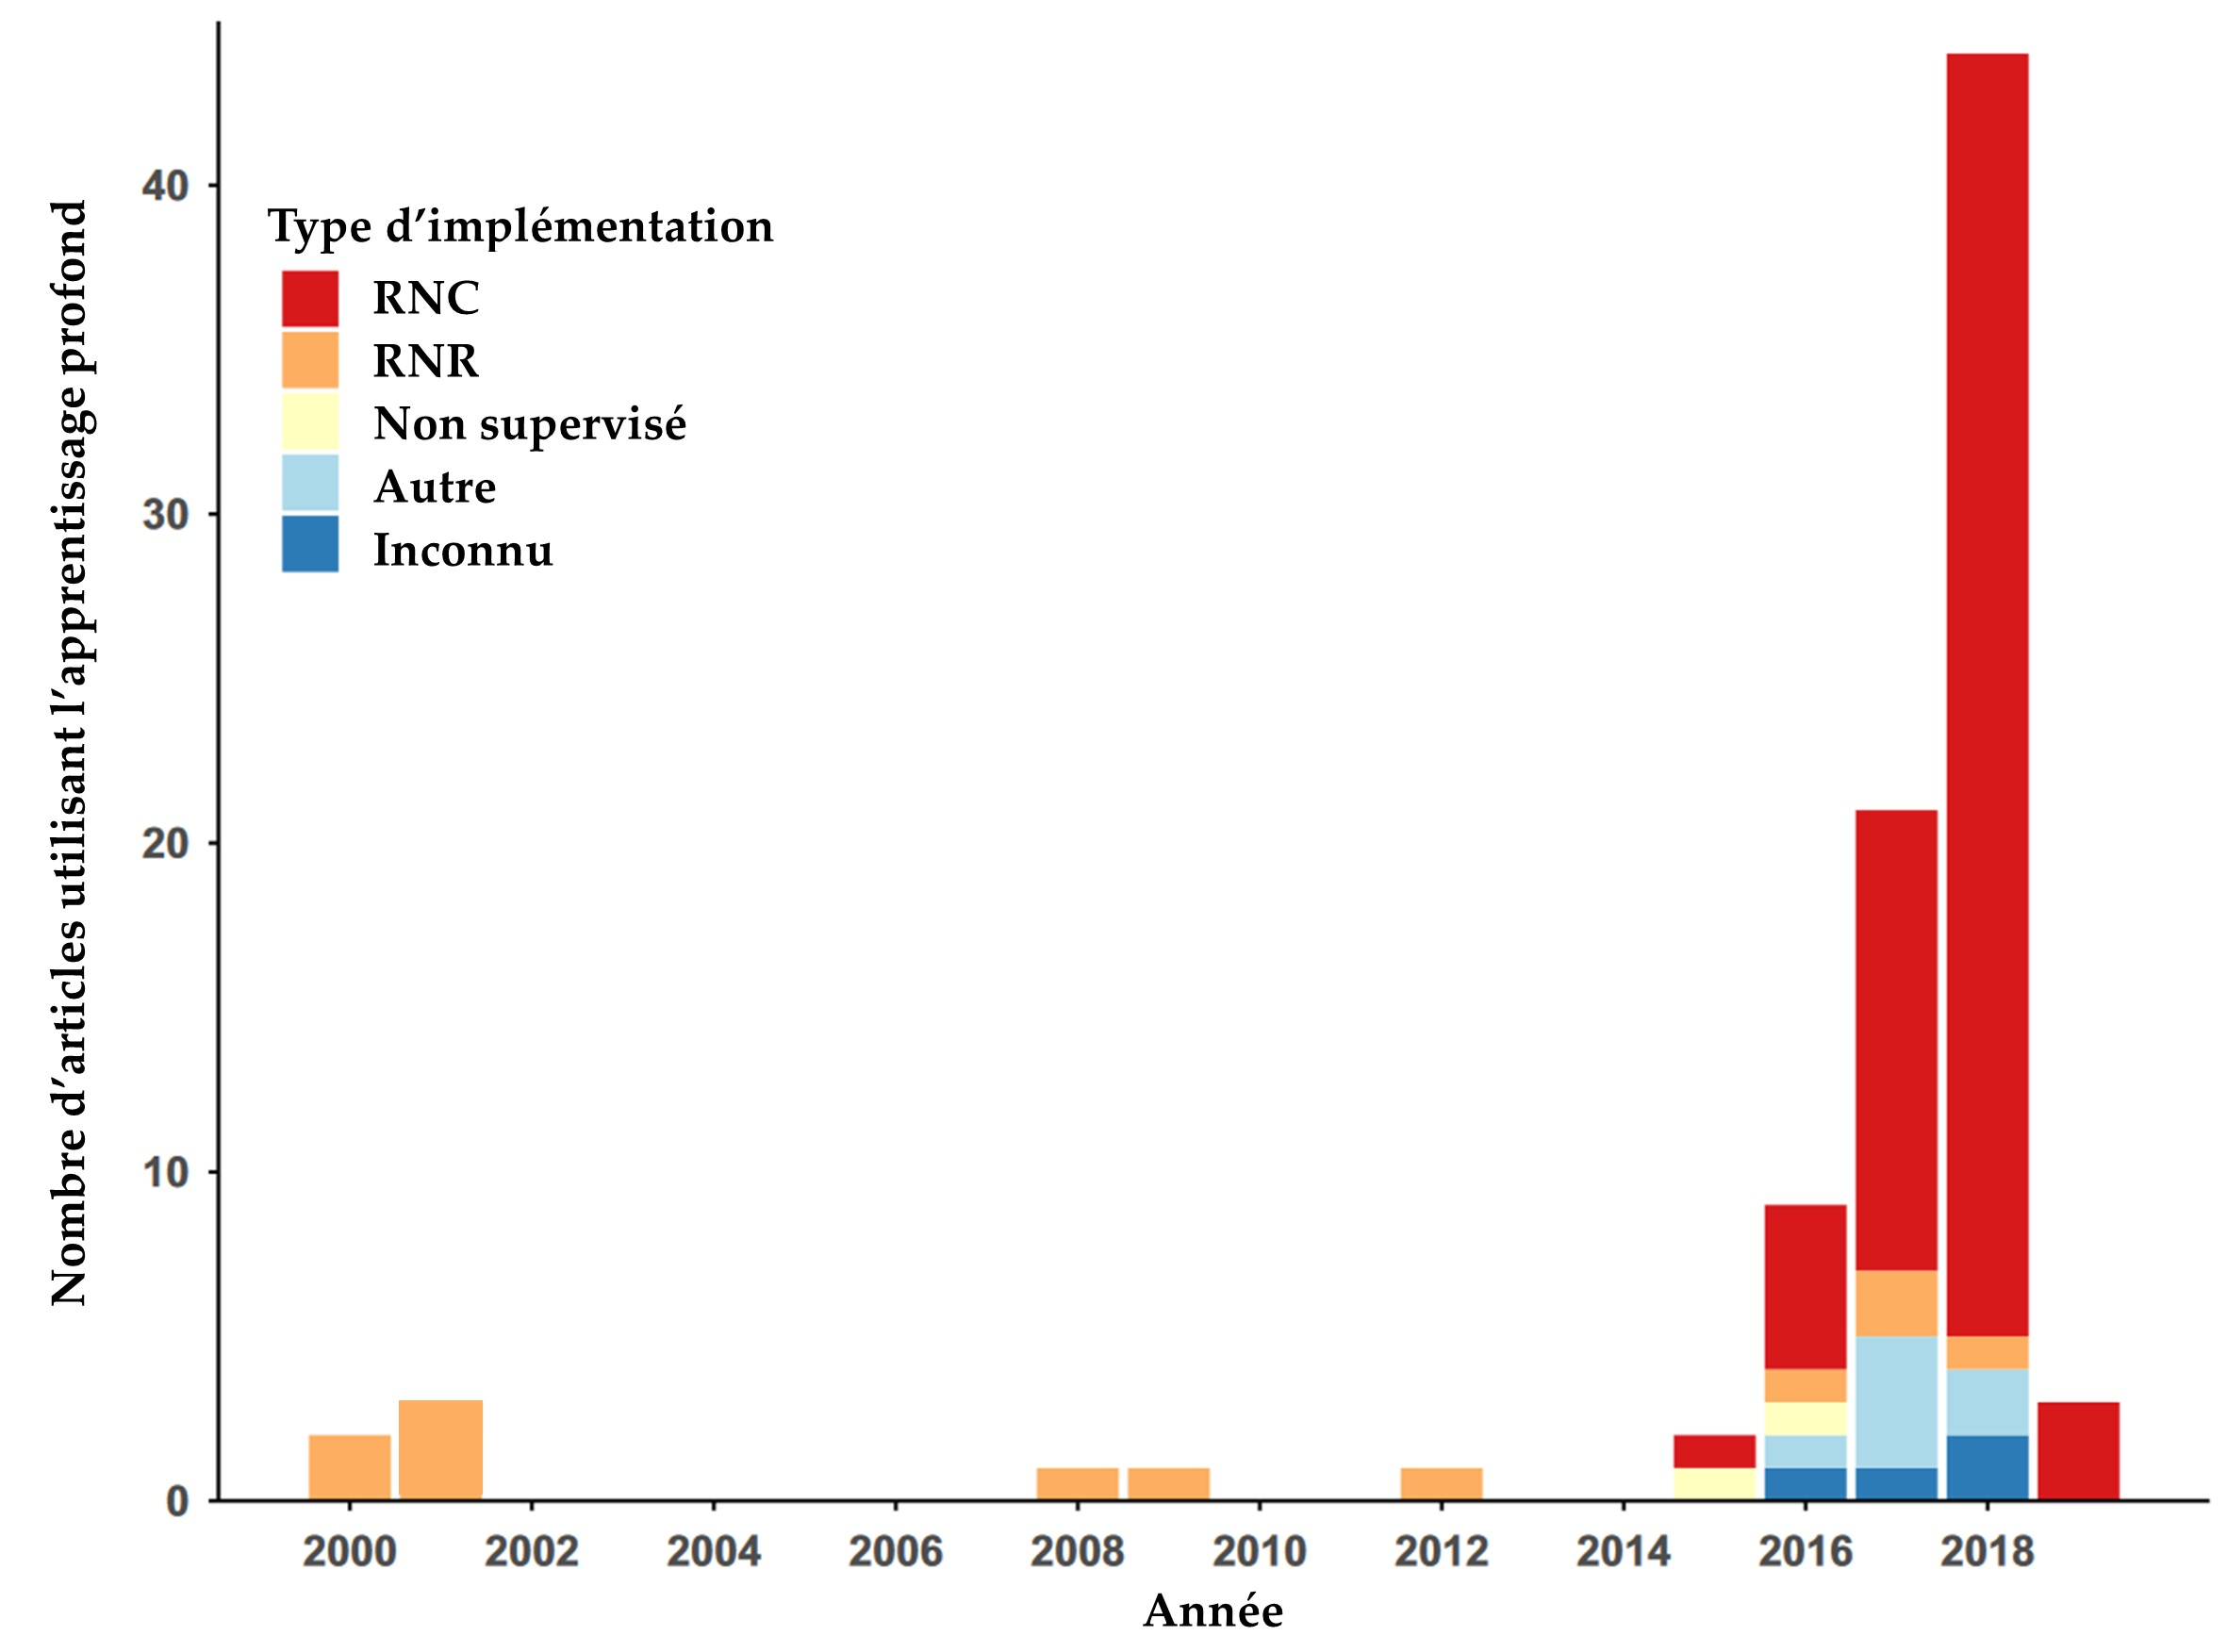
\includegraphics[width=0.7\linewidth,keepaspectratio]{./2_methodes/CNN_ecology}
		\caption[Utilisation d’algorithmes à apprentissage profond en écologie]{Utilisation d’algorithmes à apprentissage profond en écologie (adapté de \citet{christin_applications_2019}). RNC = Réseau de Neurones Convolutifs, RNR = Réseau de Neurones Récurrent.}
	\label{figure_methodo5}
\end{center}
\end{figure}

Si les RNC ont prouvé leurs redoutables performances sur des jeux de données bien particuliers avec des classes distinctes, les applications à des cas plus complexes comme la reconnaissance d’espèces soulèvent de nouveaux problèmes. Dans le cas d’images sous-marines en particulier, la variabilité des conditions lumineuses ainsi que la diversité morphologique intraspécifique des espèces benthiques rendent la tâche de classification particulièrement complexe \citep{beijbom_automated_2012}. Pour autant, les RNC ont déjà prouvé à plusieurs reprises qu’ils étaient appropriés pour la reconnaissance d’images benthiques \citep{raphael_neural_2020}. En particulier, la reconnaissance d’images de coraux par des RNC a atteint de très bonnes performances, notamment la discrimination entre corail / non corail \citep{manderson_robotic_2017, williams_leveraging_2019}. Ils ont également atteint 90 \% de bonnes classifications pour un problème à 10 classes de corail et substrat \citep{king_comparison_2018}, et il existe aujourd’hui un réseau entraîné sur un grand jeu de données d’images annotées de récifs coralliens, capable de reconnaître les principales espèces de corail : CoralNet \citep{beijbom_towards_2015}. Ce projet collaboratif s’est largement développé depuis sa création et compte aujourd’hui près de 50 000 000 d’annotations expertes sur 1 362 000 images issues de 1 451 sources à travers le monde (\autoref{figure_methodo6}).

%%%%%%%%%%%%%%%%%%%%%%%%%%%%%%%%%%%%%%%%%%%%%%
%%% Figure methodo6: Cartographie coralNet %%%
%%%%%%%%%%%%%%%%%%%%%%%%%%%%%%%%%%%%%%%%%%%%%%
\begin{figure}[H]
	\begin{center}
	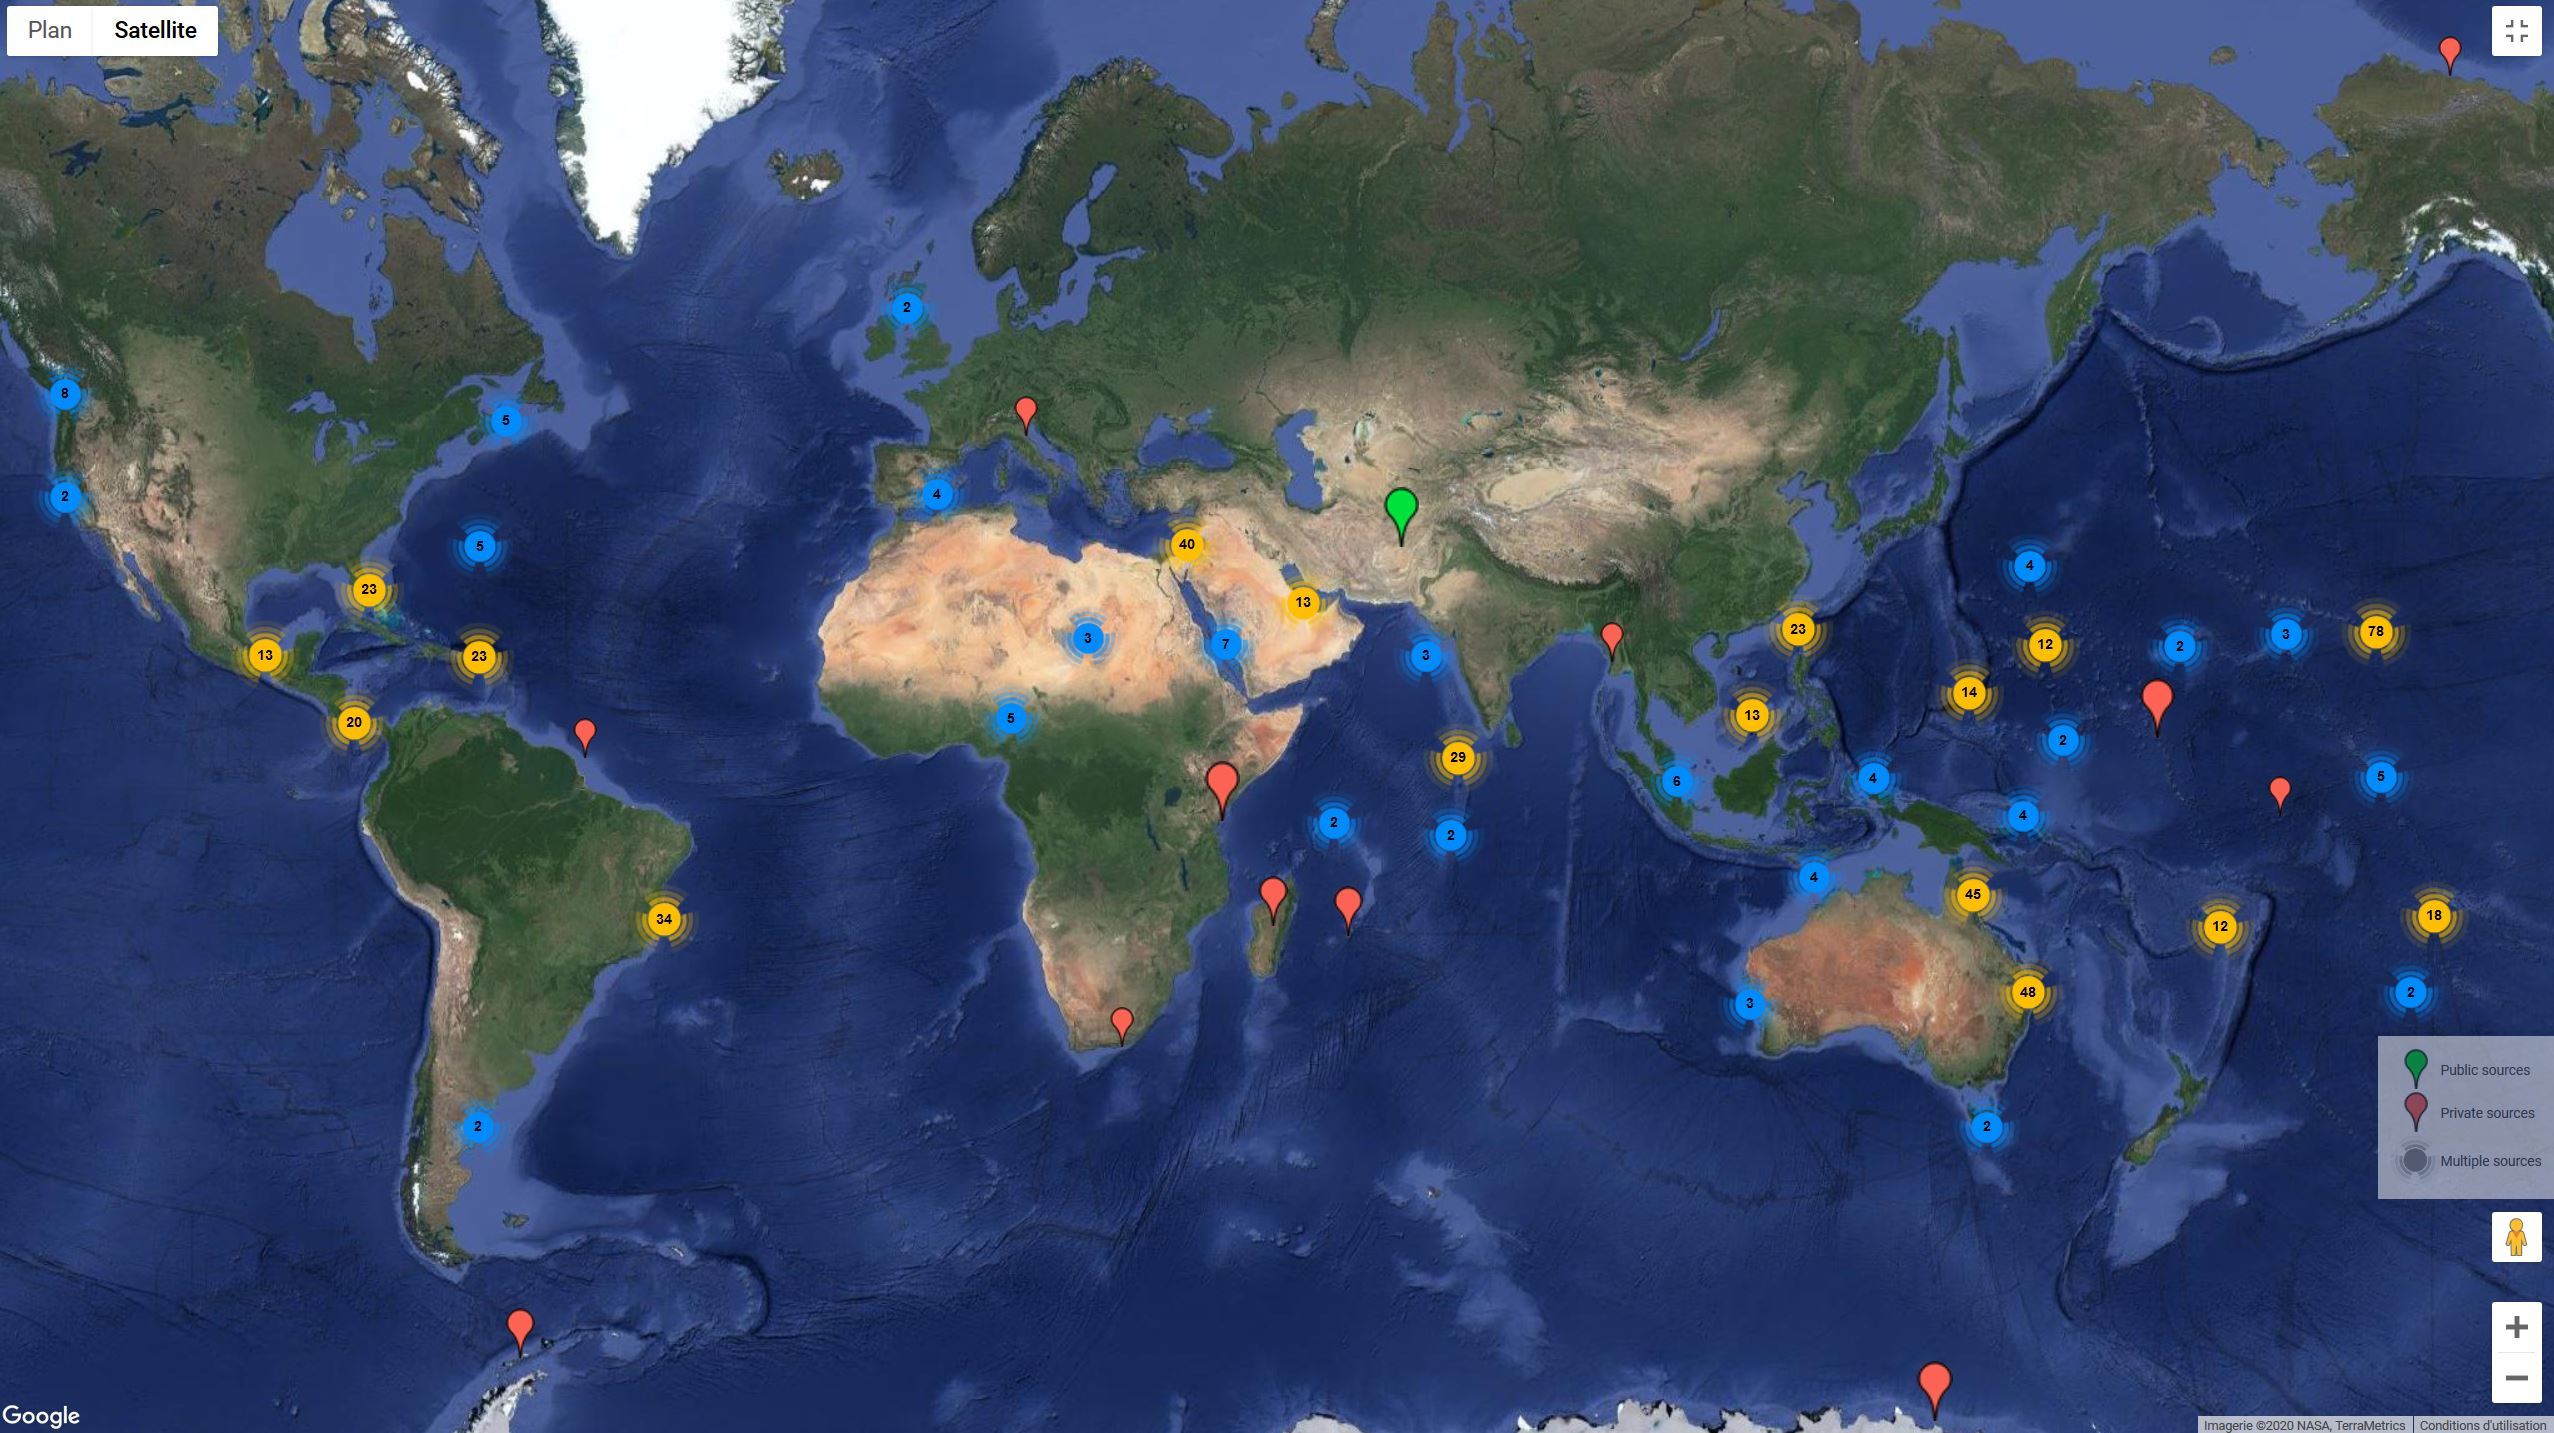
\includegraphics[width=\linewidth,keepaspectratio]{./2_methodes/coralnet_map}
		\caption[Localisation des sources d’images utilisées par CoralNet]{Localisation des sources d’images utilisées par CoralNet (source : coralnet.ucsd.edu).}
	\label{figure_methodo6}
\end{center}
\end{figure}

\setlength{\fboxsep}{5pt}
\setlength{\fboxrule}{0.6pt}
\noindent\framebox{%
  \begin{minipage}{\linewidth}
    Les RNC sont de \textbf{puissants algorithmes} permettant d’\textbf{analyser} et \textbf{interpréter} le contenu d’images de \textbf{natures très différentes}. Depuis 2015, ils sont de plus en plus utilisés en écologie, notamment en \textbf{écologie marine} pour \textbf{l’identification d’images benthiques}, où ils ont prouvé leur capacité à identifier avec précision \textbf{plusieurs catégories de substrat} et de \textbf{corail}. Ces résultats ont motivé l’entraînement d’un RNC pour la reconnaissance d’espèces du \textbf{coralligène} dans le cadre du réseau RECOR, qui est un habitat de complexité similaire aux récifs coralliens, pour lesquels aucune application de RNC n’a été décrite à ce jour.
  \end{minipage}
}

\newpage

\section[La photogrammétrie sous-marine : principes et contraintes]{La photogrammétrie sous-marine : principes et contraintes}\label{methodes.2}

\subsection{Définition}

Il existe de nombreuses situations et applications pour lesquelles il est nécessaire de mesurer des coordonnées, des distances, des surfaces ou encore des volumes. Pour les cas les plus triviaux, un simple outil de mesure peut suffire, mais il existe de nombreux cas où cela ne permet pas de réaliser les mesures souhaitées : surface complexe, précision importante requise, impossibilité de venir au contact de l’objet d’étude, taille de l’objet, ou encore la nécessité de figer un objet amené à disparaître. L’utilisation de photographies en télédétection peut répondre à certains de ces besoins plus complexes, mais leur analyse se limite à la détermination de coordonnées 2D. Afin d’obtenir des coordonnées en 3D, il faut utiliser d’autres méthodes telles que le LiDAR (laser), l’échosondeur, ou encore la photogrammétrie.

La photogrammétrie, ou « science de la mesure sur photos » \citep{linder_digital_2016}, est une technique permettant aujourd’hui de reconstruire en 3D un objet ou une scène à partir d’un grand nombre de photos prises sous différents angles de vue. Son principe de fonctionnement se base sur la vision stéréoscopique dont nous sommes nous-mêmes dotés : si nous disposons de deux (ou plus) images d’un même objet prises en différents points de vue, il est possible de calculer les coordonnées 3D de tout point de l’objet qui est visible sur les deux images. Contrairement à d’autres techniques de télédétection comme le LiDAR ou le sonar, la photogrammétrie permet de renseigner également sur la couleur et de produire un modèle de surface 3D coloré réaliste. Par la même occasion, elle permet de documenter la scène avec les mêmes images utilisées pour la reconstruction, ce qui lui confère un avantage supplémentaire. En revanche, de même qu’une image n’est qu’une représentation de la réalité, simplifiée par discrétisation (pixels) et par quantification (nombre fini de pixels différents), la photogrammétrie permet de reconstruire un « modèle 3D » qui n’est jamais qu’une représentation simplifiée de la réalité et repose sur certaines hypothèses. Par ailleurs, la photogrammétrie présente plusieurs limites qui peuvent orienter certains besoins vers d’autres méthodes d’acquisition 3D : elle nécessite une source de lumière, elle est dépendante de la visibilité et sensible aux occlusions, elle ne permet pas de capturer des objets en mouvement à l’aide d’un seul capteur, sa précision peut être parfois inférieure à celle d’autres méthodes telles que le LiDAR…

La photogrammétrie a connu un important essor ces dernières années grâce à l’amélioration des algorithmes et à l’explosion de la puissance de calcul, notamment via l’utilisation des cartes graphiques (GPU). Par ailleurs, la force des algorithmes actuels capables d’auto-calibrer les paramètres optiques de l’appareil photo durant le processus de reconstruction \citep{forstner_photogrammetric_2016} permet d’utiliser à peu près n’importe quel appareil photo pour les reconstructions, bien que la qualité du capteur et de l’optique influencent la qualité de la reconstruction \citep{linder_digital_2016}. Elle est aujourd’hui utilisée pour de nombreuses applications, depuis l’architecture et l’urbanisme jusqu’à l’écologie, en passant par l’industrie, le cinéma, l’archéologie, la géologie, la reconstruction de scènes de crime… (\autoref{figure_methodo7}).

%%%%%%%%%%%%%%%%%%%%%%%%%%%%%%%%%%%%%%%%%%%%%%%%%%
%%% Figure methodo7: Applications générales PG %%%
%%%%%%%%%%%%%%%%%%%%%%%%%%%%%%%%%%%%%%%%%%%%%%%%%%
\begin{figure}[H]
	\begin{center}
	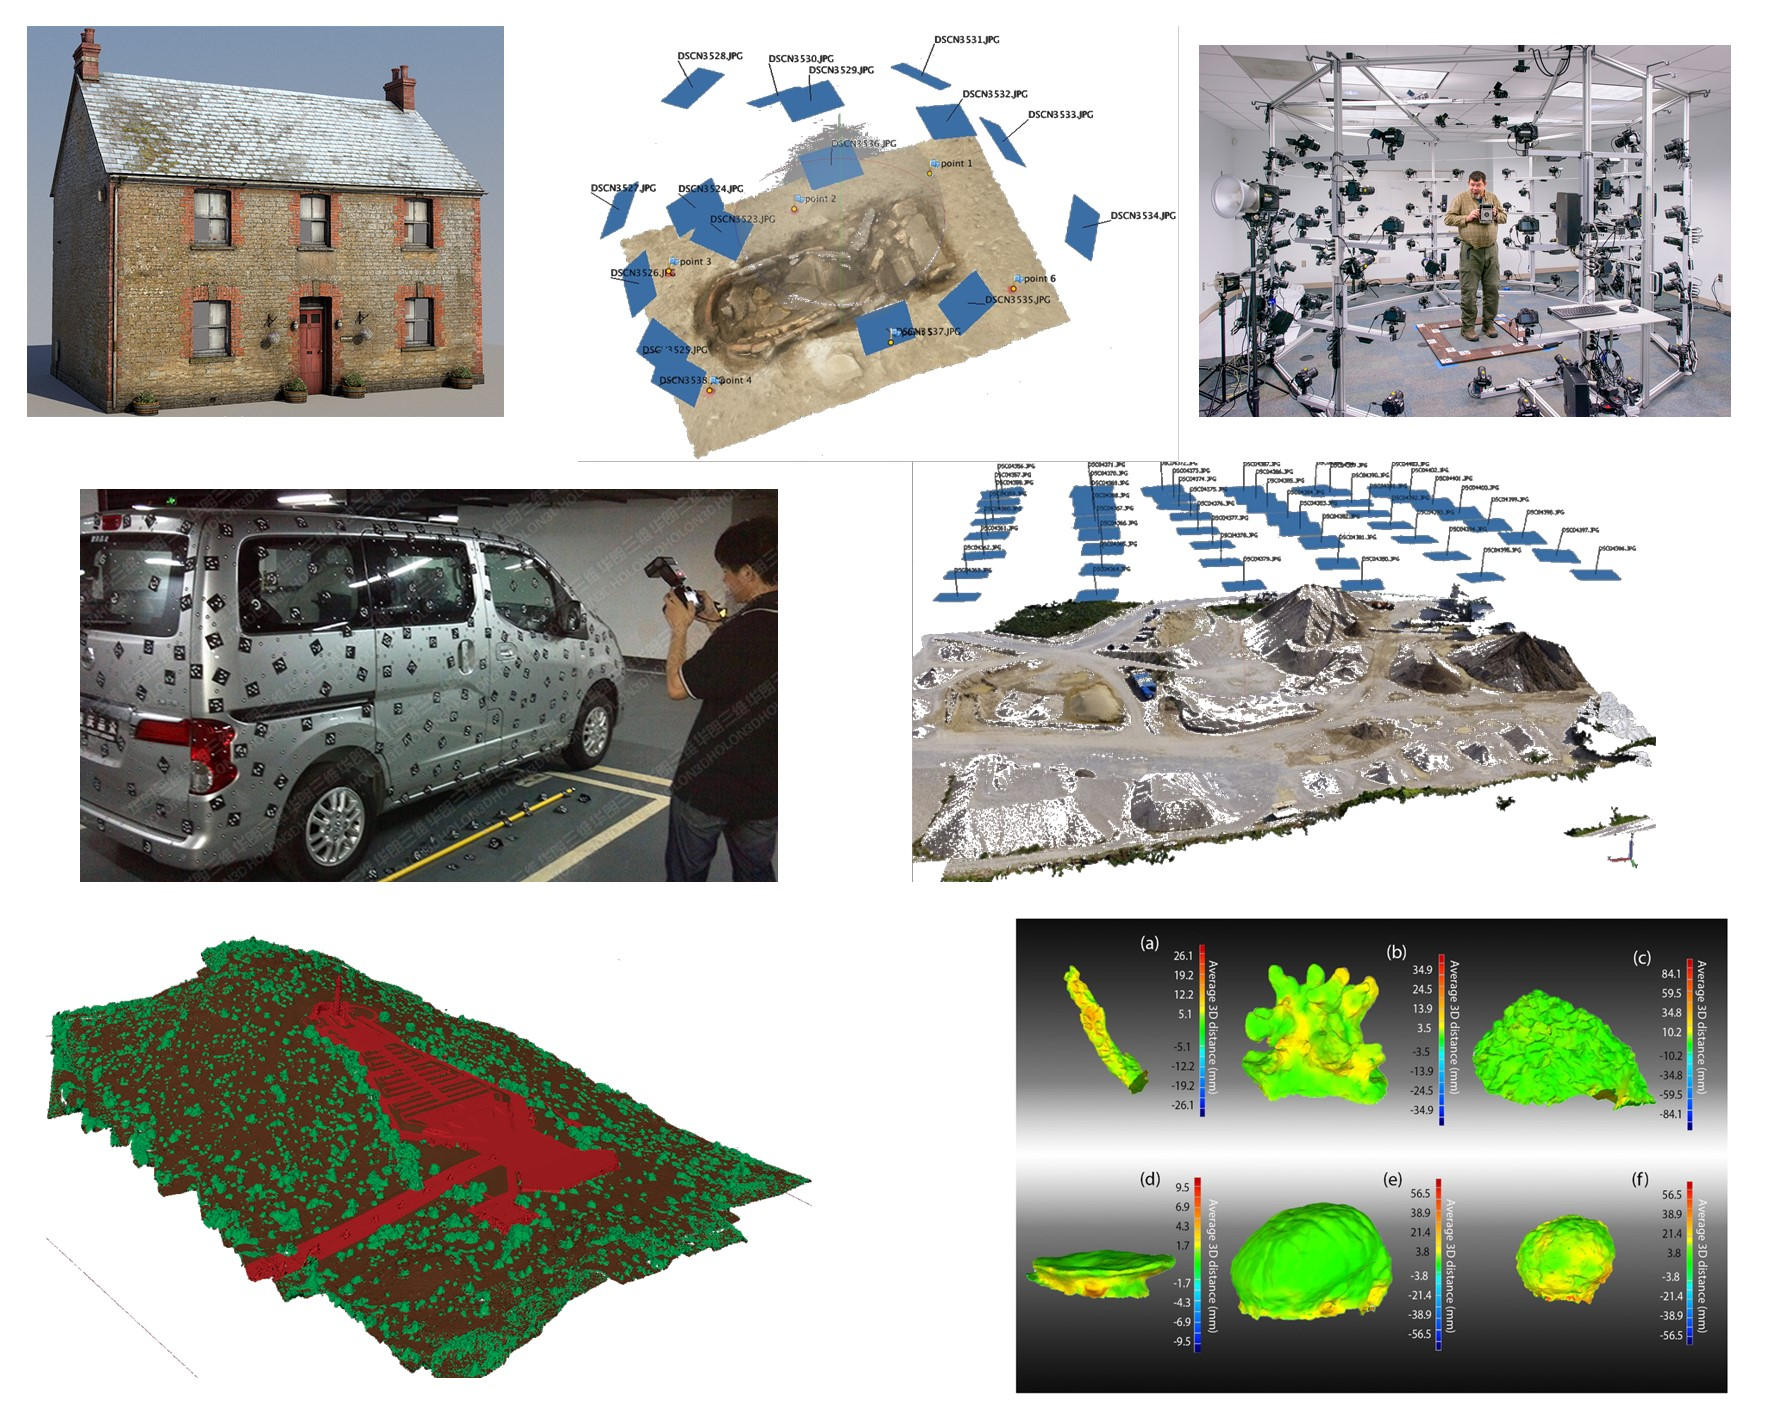
\includegraphics[width=\linewidth,keepaspectratio]{./2_methodes/applications_PG}
		\caption[Exemples d’applications de la photogrammétrie]{Exemples d’applications de la photogrammétrie. De haut en bas et de gauche à droite : architecture, archéologie, cinéma, industrie, exploitation de minerais, écologie forestière, écologie marine.}
	\label{figure_methodo7}
\end{center}
\end{figure}

\subsection{Théorie générale : les étapes de la reconstruction}

La photogrammétrie est une technique de traitement d’images qui a pour objectif la reconstruction 3D d’un objet observé sous différentes perspectives. Si à ses débuts, elle se limitait à l’interprétation manuelle de paires d’images obtenues par stéréophotogrammétrie pour reconstruire quelques coordonnées 3D et réaliser des mesures de longueur ou de hauteur, elle permet aujourd’hui d’automatiser l’ensemble du processus de reconstruction 3D de surfaces complexes. L’ensemble du processus photogrammétrique suit un enchaînement de traitements numériques pour passer des images 2D au modèle 3D (\autoref{figure_methodo8}) :

\begin{enumerate}
    \item Détection de points d’intérêt (« keypoints »)~;
    
    \item Reconnaissance des points homologues (« tie points »)~;
    
    \item Aéro-triangulation~;
    
    \item Densification du nuage de points~;
    
    \item Construction du maillage~;
    
    \item Application d’une texture.
\end{enumerate}

L’objectif de cette section n’est pas de rentrer dans le détail des calculs mathématiques associés à la reconstruction 3D, mais de fournir au lecteur une vision simplifiée permettant de comprendre le fonctionnement et l’enchaînement des différentes étapes, depuis l’analyse des images jusqu’à la production du modèle 3D réaliste.


%%%%%%%%%%%%%%%%%%%%%%%%%%%%%%%%%%%%%%%%%%%%%%%%%%%%%%%%%%%
%%% Figure methodo8: Les étapes de la reconstruction 3D %%%
%%%%%%%%%%%%%%%%%%%%%%%%%%%%%%%%%%%%%%%%%%%%%%%%%%%%%%%%%%%
\begin{sidewaysfigure}
\begin{figure}[H]
	\begin{center}
	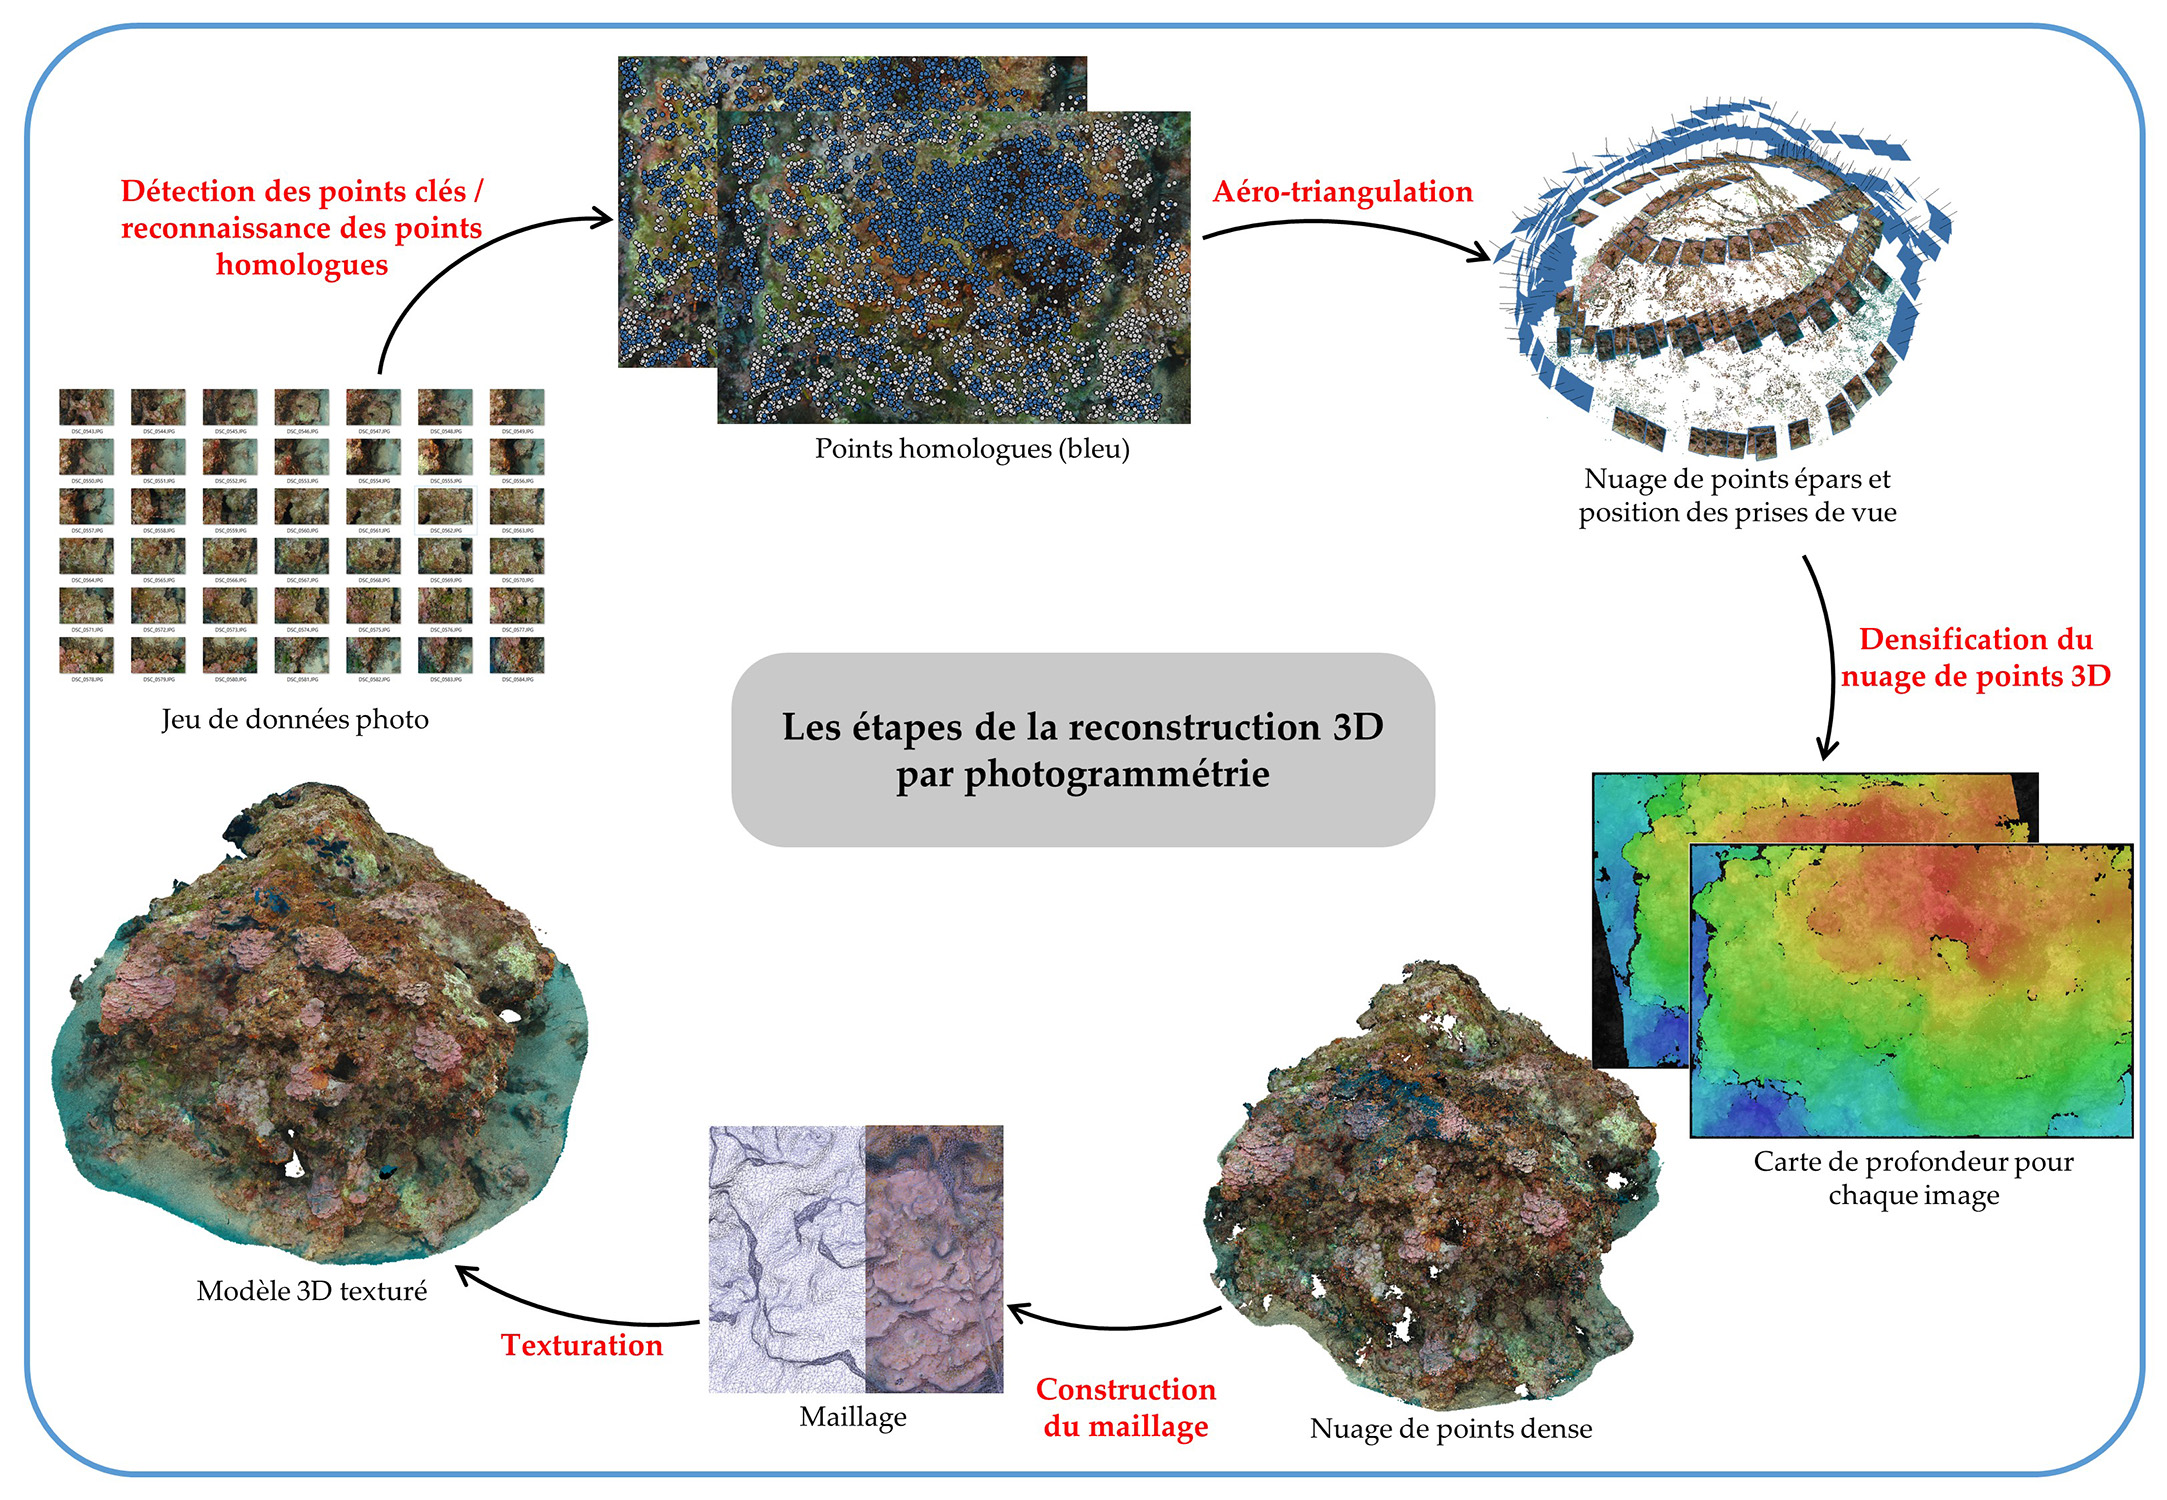
\includegraphics[width=\linewidth,keepaspectratio]{./2_methodes/encart_PG}
		\caption[Les étapes de la reconstruction 3D par photogrammétrie]{Les étapes de la reconstruction 3D par photogrammétrie.}
	\label{figure_methodo8}
\end{center}
\end{figure}
\end{sidewaysfigure}

\subsubsection{Détection des points d’intérêt (« keypoints »)}

L’ensemble des images est d’abord traité à l’aide d’un filtre afin de détecter un grand nombre de points d’intérêt sur l’image, i.e. des candidats susceptibles d’être reconnus entre deux images. Ces points clés se distinguent du reste de l’image par leur singularité : ils doivent être différents de leur voisinage, leur détection doit être robuste à de légères variations de luminosité et de contraste, ils doivent être invariants à de petites déformations géométriques, et leur détection doit être précise en X et en Y. Il existe un certain nombre de méthodes permettant de détecter ces points, mais la plus répandue est l’opérateur SIFT (pour « Scale Invariant Feature Transform »; \autoref{figure_methodo9}), car il est robuste à des différences significatives induites par une rotation, un changement d’échelle et des petites différences de perspectives entre images \citep{luhmann_close-range_2014}.

%%%%%%%%%%%%%%%%%%%%%%%%%%%%%%%%%%%%%%%%%%%%%%
%%% Figure methodo9: SIFT détection points %%%
%%%%%%%%%%%%%%%%%%%%%%%%%%%%%%%%%%%%%%%%%%%%%%
\begin{figure}[H]
	\begin{center}
	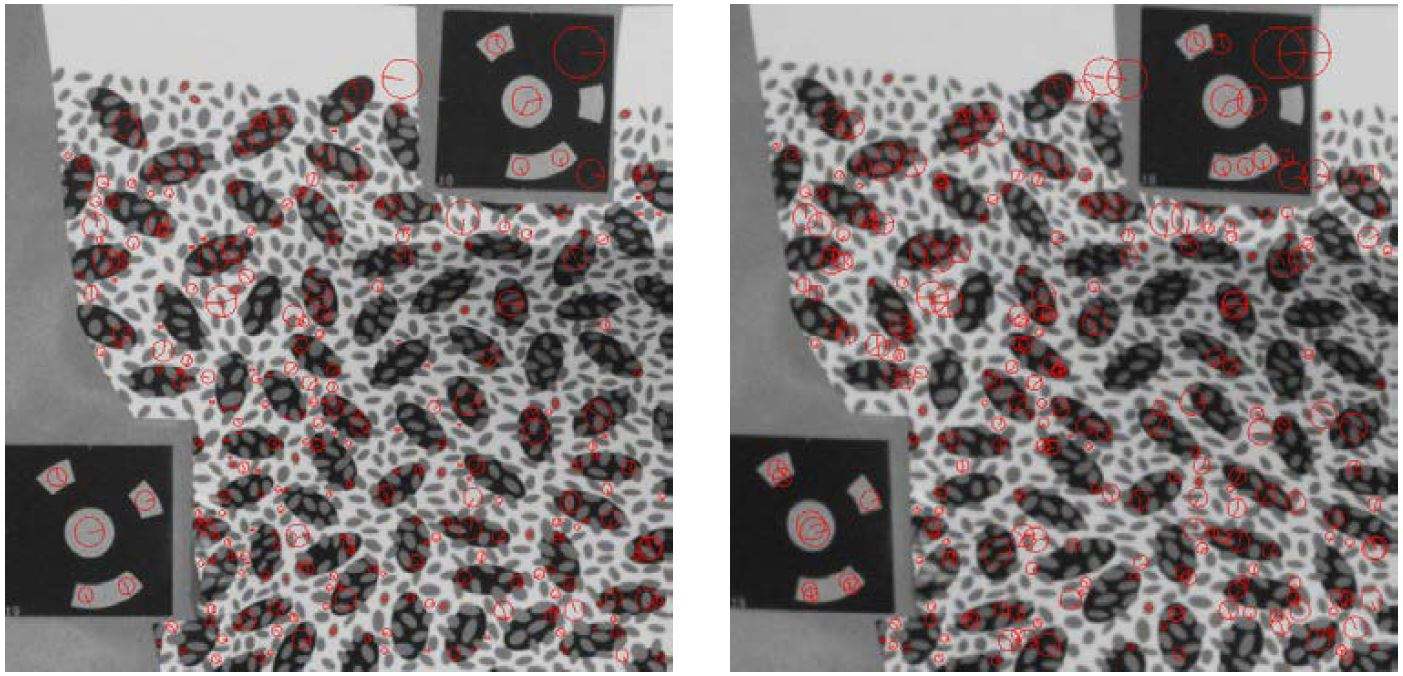
\includegraphics[width=\linewidth,keepaspectratio]{./2_methodes/SIFT_detection_Luhmann2014}
		\caption[Détection de points clés par utilisation de l’opérateur SIFT]{Détection de points clés par utilisation de l’opérateur SIFT \citep{luhmann_close-range_2014}. La taille du cercle indique à quelle échelle le point a été détecté, et la marque indique la direction du gradient dominant.}
	\label{figure_methodo9}
\end{center}
\end{figure}

Par un jeu d’opérations numériques sur l’image entière, l’opérateur SIFT permet donc de rapidement \textbf{détecter les points clés} (coordonnées XY sur l’image) et de calculer un \textbf{vecteur de descripteurs locaux} pour chaque point clé, dont les valeurs sont \textbf{invariantes à la rotation et à l’échelle}. Les descripteurs locaux correspondent à des statistiques de distribution des gradients localement calculés dans une fenêtre de 16 $\times$ 16 pixels autour du point clé. Un certain nombre de points clés sont détectés sur chaque image, en fonction de la texture de l’image (un mur blanc ne contiendra pas ou peu de points, une surface avec une texture riche et nette en contiendra davantage) avec chacun leur vecteur de descripteurs locaux associés.

\subsubsection{Reconnaissance des points homologues (« tie points »)}

Une fois les points clés détectés, il s’agit de réussir à associer les points homologues entre les images en commettant le moins d’erreurs possible, car la précision de la reconstruction 3D en dépend. Pour ce faire, l’algorithme calcule les différences entre les vecteurs de descripteurs de tous les points clés des deux images (ou plus) et associe les points dont les descripteurs sont les plus semblables (ceux dont la différence est minimale) (\autoref{figure_methodo10}). 

%%%%%%%%%%%%%%%%%%%%%%%%%%%%%%%%%%%%%%%%%%%%%%%%%
%%% Figure methodo10: SIFT association points %%%
%%%%%%%%%%%%%%%%%%%%%%%%%%%%%%%%%%%%%%%%%%%%%%%%%
\begin{figure}[H]
	\begin{center}
	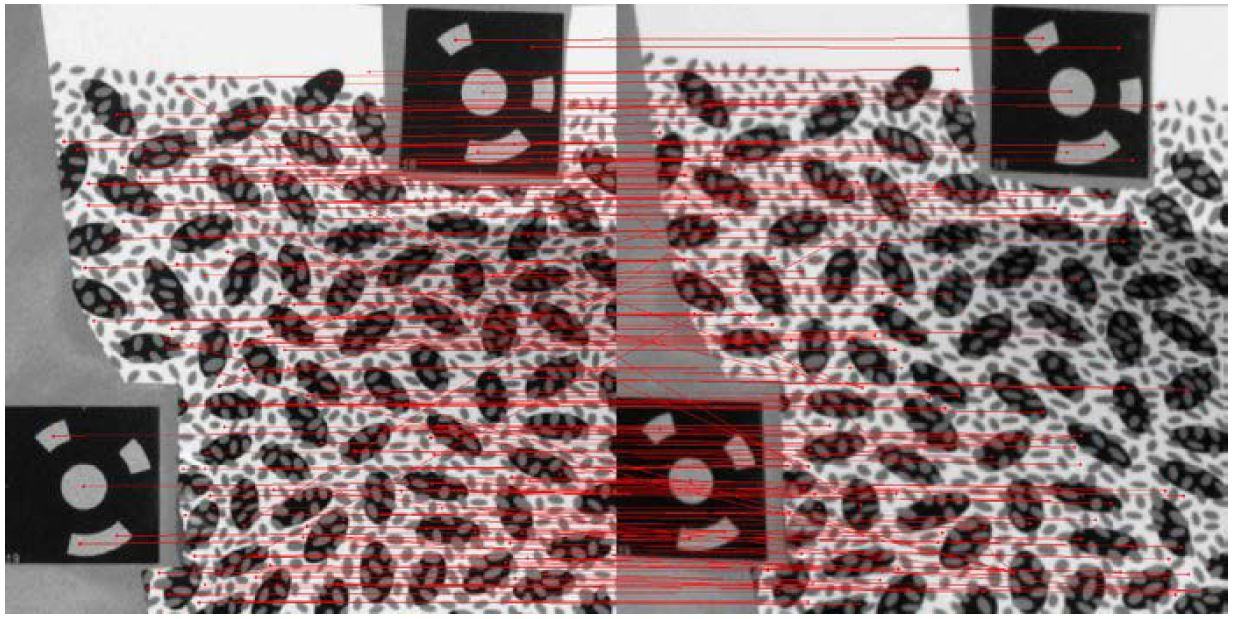
\includegraphics[width=\linewidth,keepaspectratio]{./2_methodes/SIFT_matching_Luhmann2014}
		\caption[Association des points clés détectés avec l’algorithme SIFT]{Association des points clés détectés avec l’algorithme SIFT \citep{luhmann_close-range_2014}.}
	\label{figure_methodo10}
\end{center}
\end{figure}

Cependant, une image contient souvent plusieurs points clés dont les descripteurs sont très semblables, car le même motif apparaît plusieurs fois dans l’image (par exemple : un damier, une grille…). Ceci implique qu’une certaine proportion de ces appariements est erronée, et il est important de réussir à isoler un maximum de mauvaises associations pour ne conserver que des points homologues fiables entre les images et ne pas propager l’erreur. Les erreurs sont détectées à l’aide de l’algorithme RANSAC (pour « RANdom SAmple Consensus », \citep{fischler_random_1981}) qui fonctionne de la manière suivante :

\newpage

\begin{enumerate}
    \item Sélection aléatoire d’un petit nombre de points (nombre minimal suffisant pour estimer les paramètres de l’orientation entre les images)~;
    
    \item Calcul de l’orientation relative des images sur la base de ces points (donc estimation des paramètres d’orientations internes et externes, cf. sous-partie suivante « aéro-triangulation »)~;
    
    \item Parmi les points non sélectionnés, mesure du nombre de points en accord avec l’estimation de l’orientation calculée sur le petit échantillon (avec une marge d’erreur acceptable, par exemple un pixel)~;
    
    \item Répétition des points 1-3 un grand nombre de fois ; le modèle retenu est celui permettant de maximiser le nombre de points en accord avec le modèle. Les couples de points qui s’en écartent trop sont considérés comme de fausses associations.
\end{enumerate}

Cet algorithme permet de supprimer efficacement les faux points homologues, mais le nombre d’itérations nécessaires pour s’assurer de trouver le meilleur modèle augmente avec la proportion de faux points homologues et explose littéralement avec le nombre de paramètres à estimer. Cet algorithme est utilisé dans de nombreux problèmes d’associations d’images (photogrammétrie, assemblages panoramiques, positionnement de robots par image…) et reste efficace tant que le modèle optique à construire n’excède pas une dizaine de paramètres.

\subsubsection{Aéro-triangulation}

\textbf{L’aérotriangulation} correspond au problème de \textbf{positionnement des points 3D} visibles sur une séquence d’images, et à l’estimation des paramètres \textbf{internes} (paramètres de calibration optique de l’appareil photo) et \textbf{externes} (positionnement et rotation des prises de vue). Dans le cas d’une reconstruction à partir de plusieurs images (généralement un grand nombre d’images N), la méthode utilisée est le \textbf{« bundle adjustment »}. Cette méthode permet de simultanément estimer la position et rotation des images ainsi que les positions 3D des points observés, en minimisant l’erreur de reprojection de l’ensemble des points 3D et des images par une approche des moindres carrés \citep{forstner_photogrammetric_2016}. Les inconnues de cette équation sont :

\begin{itemize}
    \item Localisations XYZ des points 3D ($3 \times K$ (points) paramètres)
    
    \item Facteur d’échelle (1 paramètre)
    
    \item Paramètres externes de chaque image (coordonnées $XYZ$ + 3 angles de rotation = 6 paramètres)
    
    \item Paramètres internes linéaires de l’appareil photo (appareil photo et réglages identiques pour tout le jeu de données) :
    
    \begin{itemize}
        \item $F$ : distance focale réelle du système optique
        
        \item $c_x$, $c_y$ : coordonnées d’intersection de l’axe optique principal avec le centre du capteur
        
        \item $b1$, $b2$ : coefficients d’affinité et de cisaillement (i.e. correction de la non-uniformité des échelles sur les axes X et Y)
    \end{itemize}
    
    \item Paramètres internes non linéaires (généralement négligés dans un premier temps) :
    
    \begin{itemize}
        \item $k1$, $k2$, $k3$, $k4$ : coefficients de distorsion radiale
        
        \item $p1$, $p2$, $p3$, $p4$ : coefficients de distorsion tangentielle
    \end{itemize}
\end{itemize}

Le « bundle adjustment » permet donc d’estimer précisément l’ensemble de ces paramètres à partir des points homologues détectés entre les images et de leurs coordonnées XY sur chaque image (voir partie précédente). Par exemple, dans le cas d’un jeu de données composé de 10 000 images (appareil photo et réglages identiques pour tout le jeu de données), 1 000 points par image, chaque point étant visible en moyenne sur 10 images :

\begin{itemize}
    \item \textbf{Nombre d’observations :} 2 (XY) $\times$ 10 000 (images) $\times$ 1 000 (points / image) = 20 000 000 observations
    
    \item \textbf{Nombre d’inconnues :} 1 000 000 (points 3D) $\times$ 3 (XYZ) + 10 000 (images) $\times$ 6 (paramètres externes) + 5 paramètres internes + 1 facteur d’échelle = 1 060 006 paramètres
    
    \item \textbf{Résolution :} nettement plus d’observations que d’inconnues, donc le système d’équations est théoriquement soluble.
\end{itemize}

Le bundle adjustment est statistiquement optimal dans la mesure où il exploite l’ensemble des observations pour l’estimation des paramètres et considère toutes les incertitudes (notamment l’incertitude de localisation des points homologues sur les images). En revanche, cette méthode d’optimisation nécessite une initialisation avec une première paramétrisation grossière : soit par des informations externes (localisation GPS, orientation par une centrale inertielle, calibration optique), soit par l’alignement séquentiel des images pour obtenir un positionnement approximatif. Si chaque point 3D doit apparaître a minima sur deux images pour pouvoir être reconstruit, il faut au moins quatre observations par point pour détecter et identifier une erreur grossière d’appariement (objet répété dans l’espace reconstruit, objet en mouvement…).

\subsubsection{Densification du nuage de points 3D}

A ce stade de la reconstruction, le nuage de points 3D produit par la reconnaissance de points homologues et le bundle adjustment est très peu dense (« sparse point cloud »), car seuls les points saillants qui se distinguent de leur voisinage sur les images ont été détectés comme points d’intérêt et associés entre images. Pour produire un nuage de points dense, capturant un maximum de détail de la scène 3D reconstruite, il est nécessaire d’associer autant que faire se peut chaque pixel d’une image à un pixel d’une autre image (ou de plusieurs images). Afin de réduire l’espace de recherche des points homologues pour chaque pixel, les algorithmes utilisent la « contrainte épipolaire » \citep{forstner_photogrammetric_2016} : à partir de la position relative de deux images, il est possible de définir pour chaque pixel d’une image la ligne épipolaire contenant les seules positions possibles du pixel homologue sur l’autre image (\autoref{figure_methodo11}). Cela permet de réduire l’espace de recherche à une seule dimension et accélère grandement les calculs. L’association des pixels homologues est faite sur la base de descripteurs locaux, de manière similaire à la détection des points homologues durant la phase initiale de la reconstruction.

%%%%%%%%%%%%%%%%%%%%%%%%%%%%%%%%%%%%%%%%%%%
%%% Figure methodo11: Epipolar geometry %%%
%%%%%%%%%%%%%%%%%%%%%%%%%%%%%%%%%%%%%%%%%%%
\begin{figure}[H]
	\begin{center}
	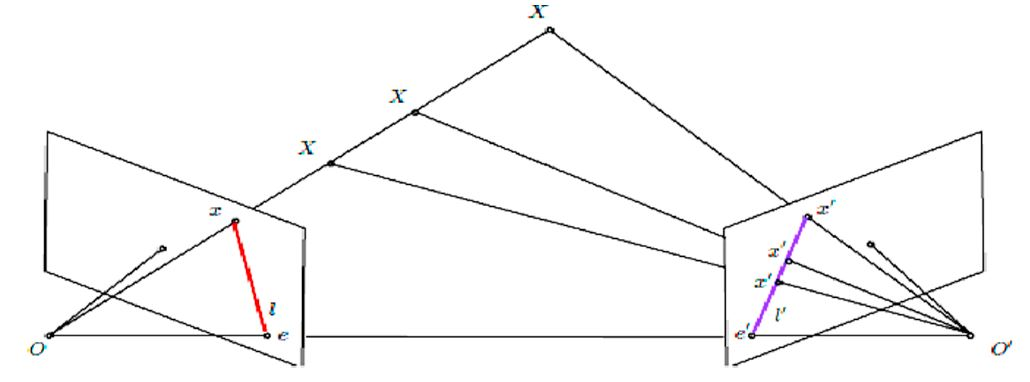
\includegraphics[width=\linewidth,keepaspectratio]{./2_methodes/epipolar_geometry}
		\caption[Illustration de la géométrie épipolaire]{Illustration de la géométrie épipolaire \citep{emmanouil_comparison_2015}. $O$ et $O^\prime$ deux images, $x$ et $x^\prime$ les projections du point $X$ sur les deux images ; $e$ et $e^\prime$ les épipoles de chaque image ; $l$ et $l^\prime$ les lignes épipolaires des deux images.}
	\label{figure_methodo11}
\end{center}
\end{figure}

Pour chaque pixel de chaque image, la distance à l’objet est calculée à partir des associations précédemment faites et de l’orientation relative des images. Il en résulte une carte de profondeur (distance à l’objet en chaque pixel) pour chaque image, à partir desquelles il est possible de déterminer les coordonnées 3D de l’ensemble des pixels pour construire le nuage de points dense. Le résultat est généralement bruité par de mauvaises associations ou de légères erreurs de positionnement, mais des algorithmes permettent de filtrer les points isolés ayant de grandes chances d’être des artefacts de reconstruction.

\subsubsection{Construction du maillage}

Le nuage de points dense est ensuite drapé par une surface 3D (i.e. maillage ou « mesh ») sur laquelle pourra être projetée la texture issue des images. L’objectif est de définir une surface 3D continue qui passe au plus proche de l’ensemble des points du nuage de points dense, en reproduisant le plus fidèlement les détails de la scène sans conserver les petits artefacts de reconstruction du nuage de points dense. Plusieurs algorithmes existent, mais le plus connu et utilisé est certainement l’algorithme de reconstruction de surface de Poisson \citep{kazhdan_poisson_2006}. Le maillage ainsi produit est constitué de faces et de sommets qui interconnectent les faces entre elles. Les faces sont généralement triangulaires mais il est aussi possible de définir des faces quadratiques (parallélépipèdes).

\subsubsection{Application d’une texture}

La texture correspond aux motifs observés sur une surface et dus aux variations de structure et de couleur dans un voisinage restreint. Cette apparence de l’objet est le résultat des propriétés de réflexion du matériau ainsi que des caractéristiques géométriques locales de la surface. Si cette étape n’est pas indispensable au processus de reconstruction 3D, l’application d’une texture au maillage permet de donner une apparence réaliste aux reconstructions 3D et de mieux visualiser l’objet reconstruit \citep{luhmann_close-range_2014}. Il existe plusieurs manières de procéder, mais bien souvent la texture associée à un chaque face du maillage est extraite de l’image qui la représente le mieux (i.e. l’image la plus orthogonale à la face, la plus proche, la mieux exposée…).

\subsection{Spécificités du milieu marin}

Alors que la démocratisation des images satellites et des drones permet aujourd’hui d’avoir accès à des images aériennes de grande qualité et le plus souvent géoréférencées, une grande partie du milieu marin reste inobservable de cette manière. Dans le cas des drones, des programmes de gestion de plan de vol permettent de réaliser des acquisitions photogrammétriques parfaitement maîtrisées (ex. : Fligh Plan de la marque Parrot) et ainsi maîtriser la qualité des reconstructions, mais le milieu sous-marin étant un milieu contraignant, une fois sous la surface de l’eau, tout devient plus complexe : positionnement, visibilité…

\subsubsection{Géoréférencement indisponible}

Le signal GPS ne fonctionne pas sous l’eau, ce qui rend impossible tout positionnement absolu des images. Ce problème est bien connu des roboticiens qui travaillent sur le développement de robots autonomes. La seule manière d’obtenir une position sous l’eau est par positionnement relatif à un objet en surface de position absolue connue, ou encore par intégration des mouvements de l’objet à positionner depuis sa dernière position absolue en surface. Cette dernière option, qui utilise une centrale inertielle (contenant des accéléromètres), rencontre d’importants problèmes de dérive avec le temps, et les solutions les plus précises sont généralement très coûteuses et peu compactes.

Pourtant, le positionnement a priori des images par l’enregistrement simultané du signal GPS permet d’améliorer la qualité et la rapidité de l’aérotriangulation. En effet, les calculs peuvent souffrir d’une dérive due à l’accumulation de petites erreurs de positionnement relatif dans le cas de gros jeux de données, et l’utilisation du positionnement GPS permet de contraindre cette dérive et d’améliorer l’ajustement \citep{lhuillier_incremental_2012}. Par ailleurs, le positionnement GPS des images de la séquence permet de géoréférencer le modèle 3D produit, et donc de le mettre automatiquement à l’échelle, correctement positionné et orienté. Sans positions absolues des images, il est indispensable d’utiliser a minima des points de contrôle sur la scène afin de mettre le modèle à l’échelle et au besoin d’orienter et géoréférencer le modèle a posteriori.

\subsubsection{L’absorption lumineuse}

Bien que translucide, l’eau est 1000 fois plus dense que l’air et absorbe une grande partie de l’énergie lumineuse qui la traverse \citep{wozniak_light_2007}. Cette absorption est d’autant plus forte que la couche d’eau traversée est grande, et il ne reste plus guère de lumière passé 100 m de fond. Par ailleurs, l’absorption n’est pas homogène sur tout le spectre visible, et les rouges sont absorbés dès 20 m de fond. L’utilisation de la photogrammétrie en milieu sous-marin implique donc de se limiter aux petits fonds pour bénéficier d’un éclairement naturel suffisant, ou impose l’utilisation d’éclairages artificiels qui posent d’autres problèmes potentiels : éclairement hétérogène selon la profondeur dans l’image et pouvant perturber les algorithmes de reconstruction, ombres portées masquant certaines parties de l’image, nécessité d’une plus grande proximité à l’objet…

\subsubsection{La réfraction}

La réalisation de photos sous-marines implique l’utilisation d’un caisson étanche et donc d’une optique externe à travers laquelle la lumière pénètre dans le caisson. Les rayons lumineux qui passent de l’eau à l’air en traversant cette optique subissent une réfraction et sont déviés avant d’atteindre l’objectif de l’appareil photo et peuvent affecter le processus de reconstruction photogrammétrique \citep{telem_photogrammetric_2010}. En effet, cette réfraction cause des déformations \\géométriques et une réduction du champ de vision, c’est pourquoi il est courant d’utiliser un dôme hémisphérique plutôt qu’un dôme plan afin de compenser la réfraction et d’améliorer la qualité des reconstructions 3D (\autoref{figure_methodo12}) \citep{menna_optical_2017}. Si le système optique composé de l’objectif et de l’optique externe sous l’eau n’est pas équivalent à l’appareil l’objectif seul à l’air libre, il a été démontré que les déformations optiques résiduelles peuvent être absorbées et corrigées par l’auto-calibration réalisée pendant la phase d’aérotriangulation \citep{shortis_calibration_2015}.

%%%%%%%%%%%%%%%%%%%%%%%%%%%%%%%%%%%%
%%% Figure methodo12: Réfraction %%%
%%%%%%%%%%%%%%%%%%%%%%%%%%%%%%%%%%%%
\begin{figure}[H]
	\begin{center}
	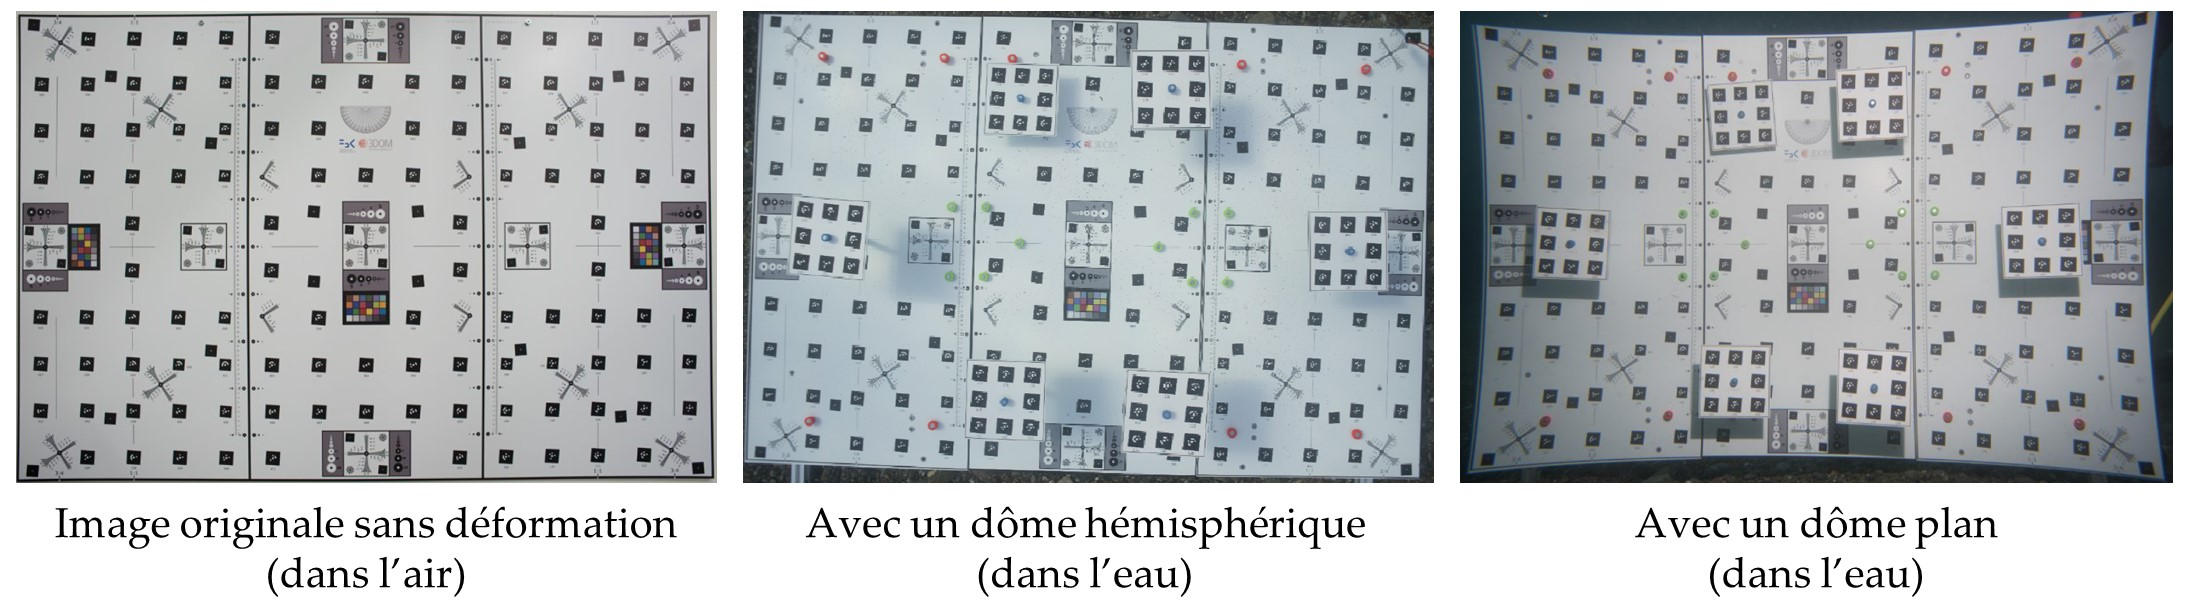
\includegraphics[width=\linewidth,keepaspectratio]{./2_methodes/refraction_Menna2017}
		\caption[Déformations optiques avec un dôme hémisphérique ou un dôme plan]{Déformations optiques avec un dôme hémisphérique ou un dôme plan (adapté de \citet{menna_optical_2017}).}
	\label{figure_methodo12}
\end{center}
\end{figure}

\subsubsection{Présence d’objets mobiles sur la scène}

Les habitats sous-marins sont peuplés d’espèces fixées soumises aux courants marins (plantes marines, algues, gorgones…) et d’espèces mobiles comme les poissons. S’ils occupent une part trop importante de l’image, ces objets en mouvement peuvent largement perturber le processus de reconstruction, qui repose à la base sur la reconnaissance de points homologues pour calculer le positionnement des images et les coordonnées 3D des points de la scène. C’est le cas particulièrement sur les récifs coralligènes où l’on rencontre régulièrement d’abondantes populations de poissons (\autoref{figure_methodo13}).

%%%%%%%%%%%%%%%%%%%%%%%%%%%%%%%%%%%%%%%%%
%%% Figure methodo13: Espèces mobiles %%%
%%%%%%%%%%%%%%%%%%%%%%%%%%%%%%%%%%%%%%%%%
\begin{figure}[H]
	\begin{center}
	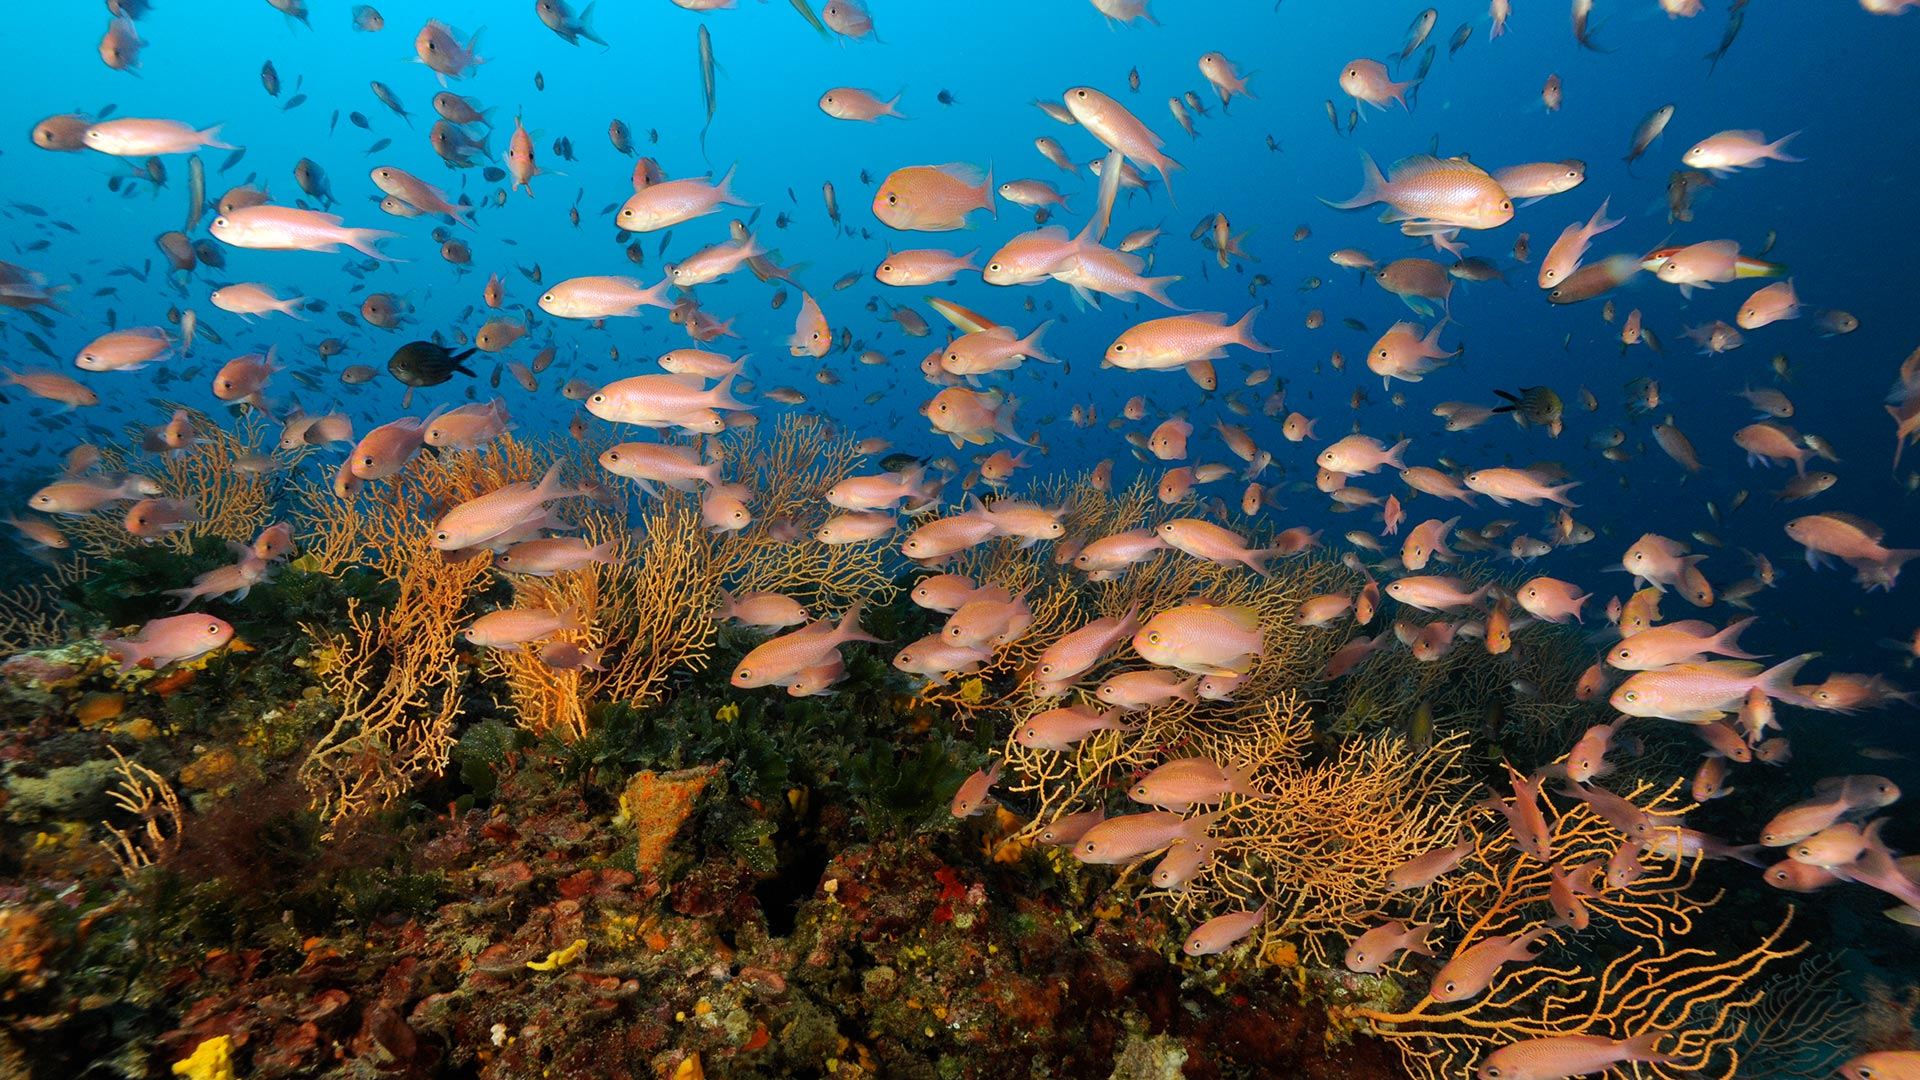
\includegraphics[width=\linewidth,keepaspectratio]{./2_methodes/especes_mobiles}
		\caption[Illustration du problème des espèces mobiles sur les images sous-marines]{Illustration du problème des espèces mobiles sur les images sous-marines. Ici de nombreux barbiers communs (\textit{Anthias anthias}) sur un récif coralligène (\textit{©Andromède océanologie}).}
	\label{figure_methodo13}
\end{center}
\end{figure}

\newpage

\subsection{La photogrammétrie en pratique}

\subsubsection{Acquisition des images}

L’acquisition des images est une étape clé pour une reproduction de qualité. L’objectif est d’assurer un recouvrement suffisant entre les images pour permettre leur bon alignement dans l’espace, avec des transformations (translation, rotation, homothétie) entre deux images que les algorithmes sauront interpréter. Il est en général recommandé de maintenir un minimum de 80 \% de recouvrement entre deux images successives (80 \% des deux images recouvrent une partie commune de l’objet) et 60 \% de recouvrement latéral (i.e. entre deux « bandes » d’images) \citep{agisoft_agisoft_2018-1} pour assurer le bon alignement des images dans l’espace. Il est bien entendu possible de recouvrir plus encore, mais un trop fort taux de recouvrement risque d’affecter significativement le temps de calcul et les besoins en mémoire, qui augmentent exponentiellement avec le nombre d’images \citep{agisoft_agisoft_2018}. Par ailleurs, la trajectoire et l’orientation des images sont importantes : il est recommandé de suivre une trajectoire localement parallèle à la surface de l’objet, et une orientation de la prise de vue perpendiculaire à celle-ci (\autoref{figure_methodo14}). Concernant la distance à l’objet, il faut respecter la règle « aussi loin que nécessaire, mais aussi près que possible » \citep{linder_digital_2016}. Il est donc important d’adapter le protocole d’acquisition à chaque type d’objet en fonction de sa forme et de la qualité de reconstruction requise.

%%%%%%%%%%%%%%%%%%%%%%%%%%%%%%%%%%%%%%%%%%
%%% Figure methodo14: Prises de vue PG %%%
%%%%%%%%%%%%%%%%%%%%%%%%%%%%%%%%%%%%%%%%%%
\begin{figure}[H]
	\begin{center}
	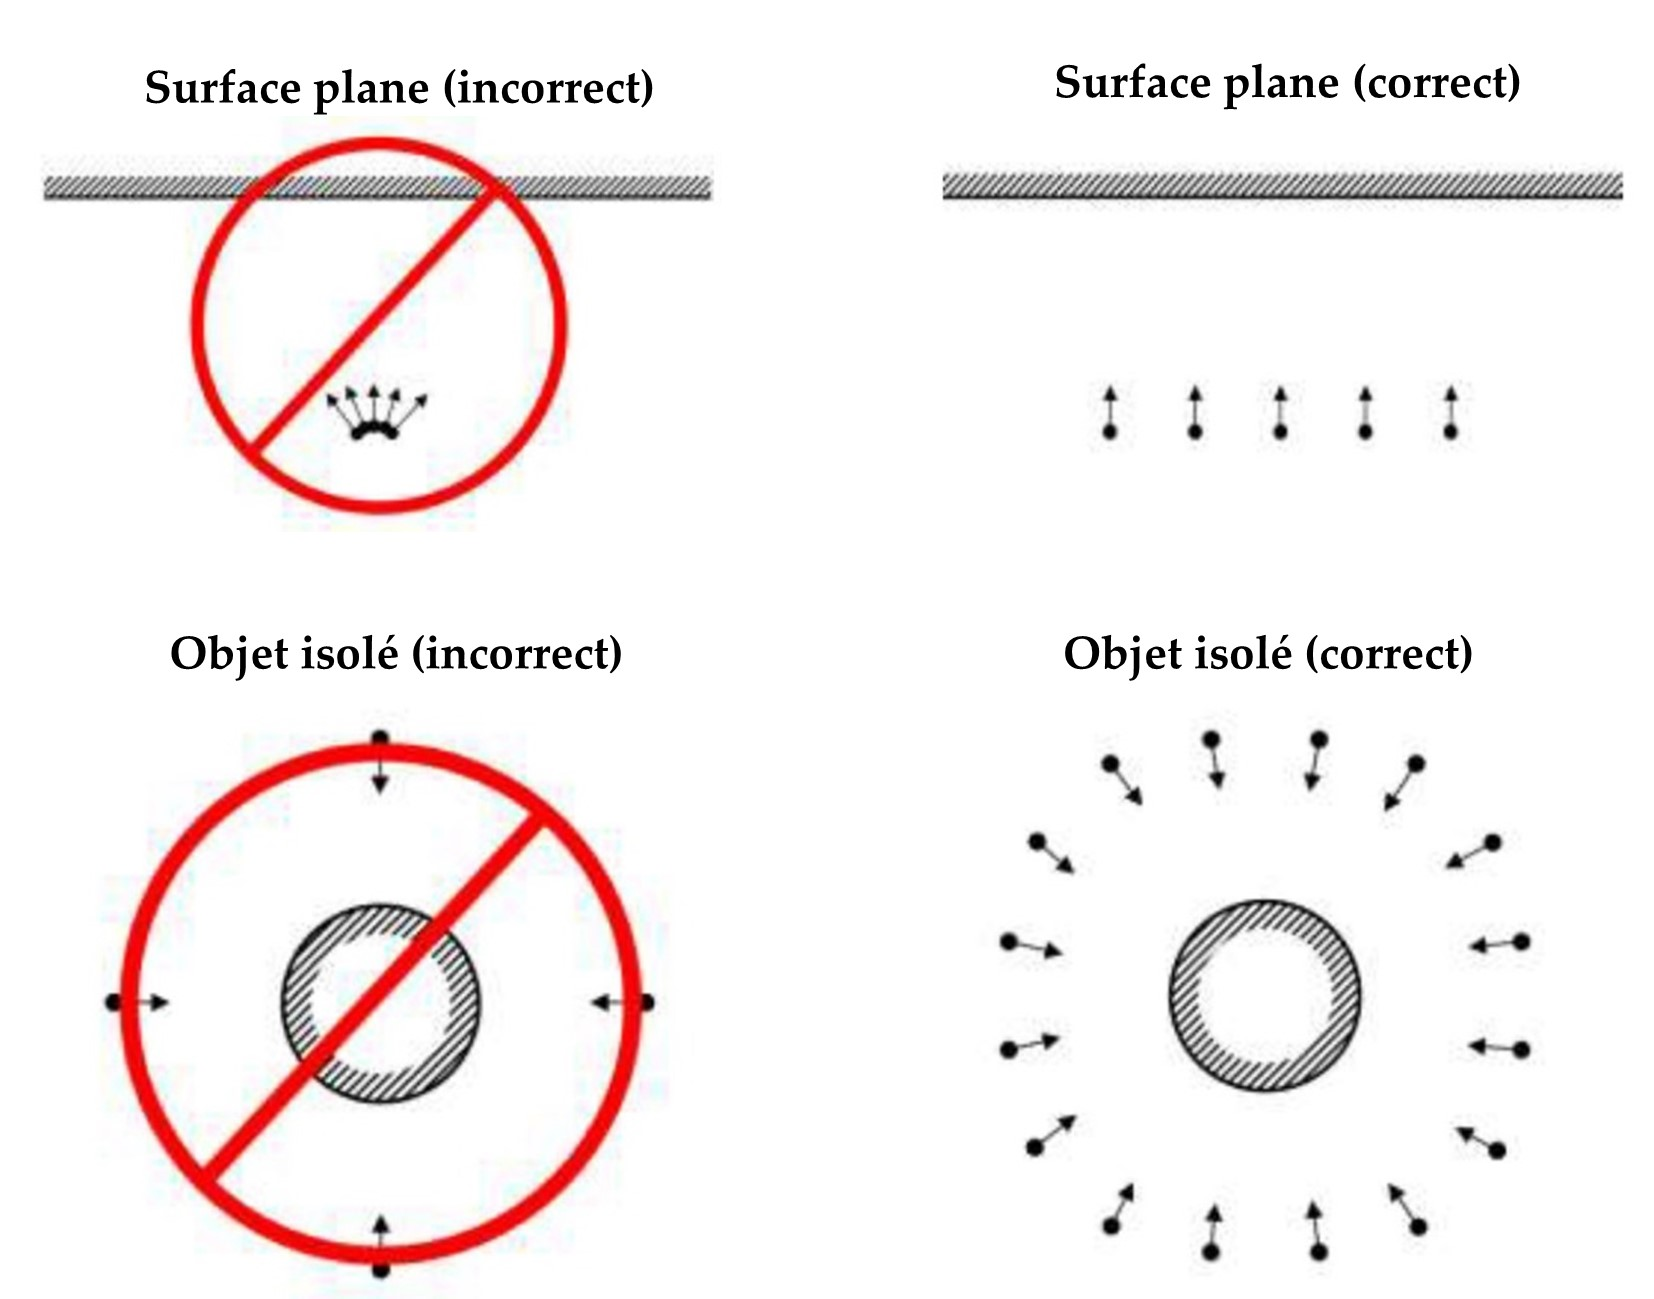
\includegraphics[width=0.7\linewidth,keepaspectratio]{./2_methodes/acquisition_PG}
		\caption[Recommandations de prises de vue pour une reconstruction 3D par photogrammétrie]{Recommandations de prises de vue pour une reconstruction 3D par photogrammétrie (adapté de \citet{agisoft_useful_2018}).}
	\label{figure_methodo14}
\end{center}
\end{figure}

La trajectoire d’acquisition dépend elle aussi de la nature et de la forme de l’objet ou de la scène à numériser. Dans le cas d’une scène relativement plane, il convient de survoler la zone en réalisant des transects parallèles, et dans le cas d’un objet plus complexe, il peut être nécessaire de suivre les courbes de niveau de l’objet en restant localement orthogonal à la surface de l’objet (\autoref{figure_methodo15}).

%%%%%%%%%%%%%%%%%%%%%%%%%%%%%%%%%%%%%%%%
%%% Figure methodo15: Trajectoire PG %%%
%%%%%%%%%%%%%%%%%%%%%%%%%%%%%%%%%%%%%%%%
\begin{figure}[H]
	\begin{center}
	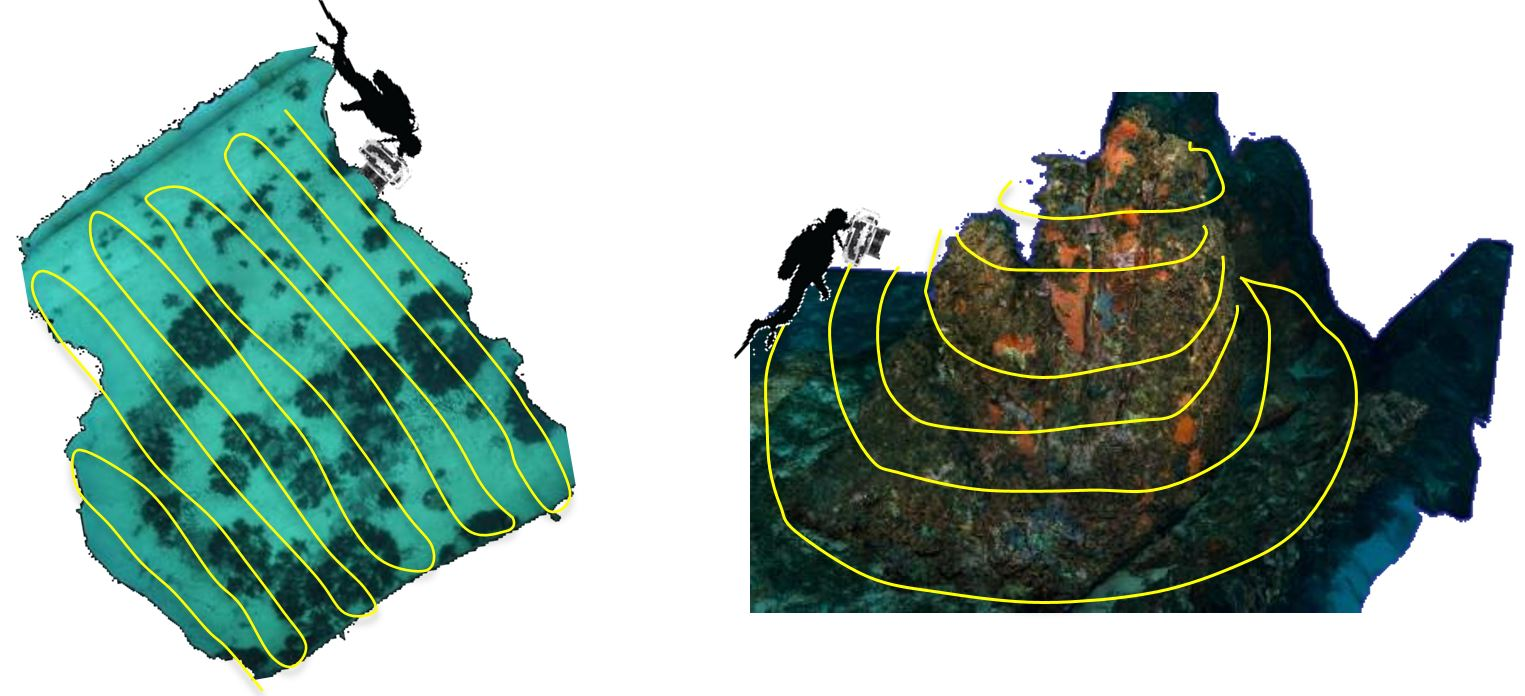
\includegraphics[width=\linewidth,keepaspectratio]{./2_methodes/trajectoire_PG}
		\caption[Exemples de trajectoires d’acquisition en fonction de la morphologie de l’objet d’étude]{Exemples de trajectoires d’acquisition en fonction de la morphologie de l’objet d’étude. À gauche : un herbier de posidonie ; à droite : un pic rocheux vertical.}
	\label{figure_methodo15}
\end{center}
\end{figure}

\subsubsection{Utilisation de points de contrôle et barres d’échelle}

L’utilisation de points de contrôle, généralement matérialisés par des marqueurs codés de coordonnées connues et automatiquement détectés par un filtre (voir exemple de marqueur \autoref{figure_methodo16}), permet de faire le lien entre le système de coordonnées arbitraire du modèle 3D après reconstruction et le système de coordonnées réel de la scène capturée \citep{forstner_photogrammetric_2016}. Chacun de ces marqueurs codés est reconnu et identifié, ce qui permet d’affecter automatiquement leurs coordonnées renseignées dans un tableau de données et facilite le géoréférencement. À défaut d’avoir à disposition les coordonnées absolues de ces marqueurs, comme c’est a priori le cas sous l’eau, il est possible de se servir des relations géographiques entre marqueurs afin de mettre à l’échelle le modèle via une barre d’échelle (distance connue entre deux marqueurs), ou même de l’orienter grâce à un référentiel local du plan XY défini par un minimum de 3 marqueurs (\autoref{figure_methodo16}).

%%%%%%%%%%%%%%%%%%%%%%%%%%%%%%%%%%%%%%%%%%%%%%%%%%%%%%
%%% Figure methodo16: Points de contrôle cibles PG %%%
%%%%%%%%%%%%%%%%%%%%%%%%%%%%%%%%%%%%%%%%%%%%%%%%%%%%%%
\begin{figure}[H]
	\begin{center}
	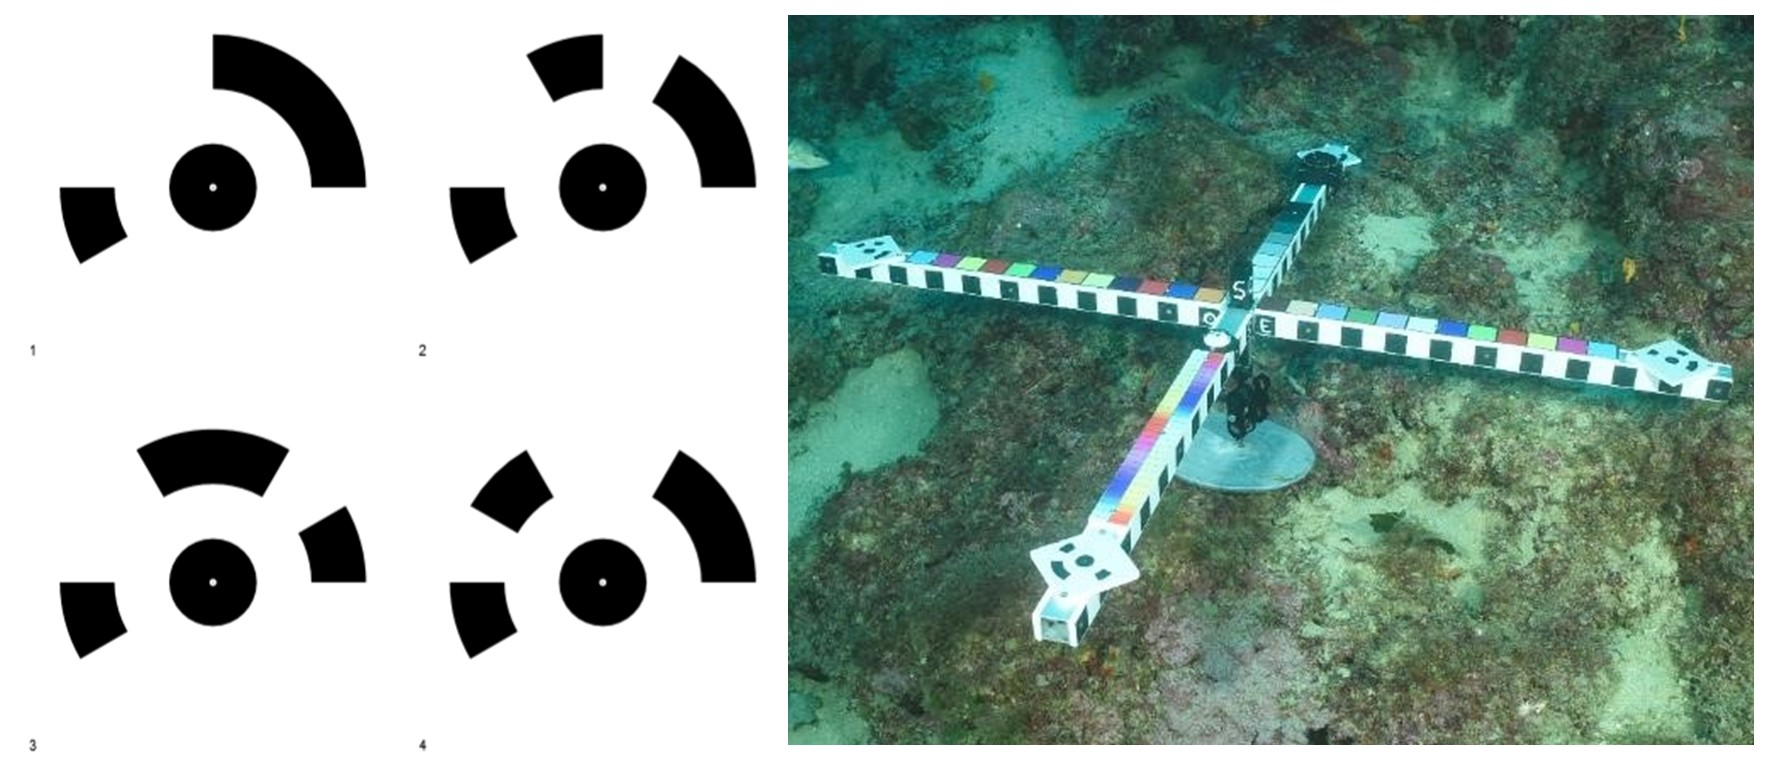
\includegraphics[width=\linewidth,keepaspectratio]{./2_methodes/marqueurs}
		\caption[Exemples de marqueurs codés utilisés par le logiciel Agisoft PhotoScan]{Exemples de marqueurs codés utilisés par le logiciel Agisoft PhotoScan. À gauche : les marqueurs codés 1-2-3-4 ; à droite : référentiel local défini par quatre marqueurs aux quatre cardinales.}
	\label{figure_methodo16}
\end{center}
\end{figure}

\subsubsection{Chaîne de traitement avec le logiciel Agisoft PhotoScan}

Les algorithmes utilisés pour l’analyse des images et la reconstruction 3D par photogrammétrie sont aujourd’hui bien connus, et de nombreux logiciels libres ou payants proposent des solutions intégrées pour utiliser ces algorithmes \citep{ioannides_benchmarking_2016}. Pour autant, toutes ces solutions logicielles ne sont pas équivalentes en précision, en robustesse, en coût, en facilité de mise en œuvre et de personnalisation des traitements. L’une d’entre elles, Agisoft PhotoScan \citep{agisoft_agisoft_2018-1}, est largement répandue et appréciée de la communauté scientifique \citep{figueira_accuracy_2015, lavy_quick_2015, burns_assessing_2016, guo_accuracy_2016, bryson_characterization_2017, casella_mapping_2017, mizuno_simple_2017, raczynski_accuracy_2017, raoult_how_2017, collin_very_2018, royer_photogrammetric_2018, ventura_mapping_2018}. En effet, PhotoScan est :

\begin{itemize}
    \item \textbf{Robuste :} il n’échoue presque jamais \citep{ioannides_benchmarking_2016} ;
    
    \item \textbf{Précis :} faibles distances entre surface réelle et reconstruite ;
    
    \item \textbf{Son coût est raisonnable :} 180 – 500 € en version académique ;
    
    \item \textbf{Intuitif :} utilisable en « clic-bouton » ;
    
    \item \textbf{Personnalisable :} grâce à une interface Python permettant de scripter des tâches complexes et d’accéder à tous les objets produits au cours du traitement.
\end{itemize}

L’ensemble des traitements photogrammétriques détaillés dans ce travail de thèse sont réalisés avec le logiciel Agisoft PhotoScan v1.4 \citep{agisoft_agisoft_2018-1}. Ci-dessous le détail des différentes étapes nécessaires à la reconstruction 3D, avec les différents paramètres à renseigner et leur signification.

\paragraph{Aligner les images}

Cette étape inclut la détection de points clés, la reconnaissance des points homologues et l’aérotriangulation des images (voir section 2.2). Elle utilise plusieurs paramètres :

\begin{itemize}
    \item \textbf{Précision de l’alignement :} plus elle augmente, meilleur est le positionnement des images, mais plus le temps de calcul est long. Lorsque l’utilisateur choisit « haute précision », les images sont traitées dans leur résolution originale. Pour chaque niveau de dégradation de la précision (i.e. « moyenne », « faible », « très faible »), la résolution originale est dégradée par un facteur 2 en X et en Y, donc le nombre de pixels de l’image est divisé par 4 ;
    
    \item \textbf{Présélection des paires d’images :} afin de réduire le temps de calcul pour les gros jeux de données, il est possible de réaliser un préalignement imprécis des images se chevauchant ou dont les coordonnées sont renseignées ;
    
    \item \textbf{Nombre maximal de points clés :} permet de contrôler le nombre de points clés détectés par les algorithmes, afin de se limiter aux points les plus fiables ;
    
    \item \textbf{Nombre maximal de points homologues :} permet de contrôler le nombre maximal de points homologues entre deux images et de réduire les erreurs en se limitant aux points clés les plus semblables entre deux images ;
    
    \item \textbf{Ajustement variable du modèle de correction optique :} autorise PhotoScan à choisir automatiquement les paramètres optiques à estimer durant la phase d’alignement. De base, seuls les paramètres suivants sont calculés : $F$, $c_x$, $c_y$, $k1$, $k2$, $k3$, $p1$ et $p2$ (voir section 2.2.3).
\end{itemize}

\paragraph{Optimiser l’alignement}

Durant la première étape, PhotoScan reconnaît les points homologues entre les différentes images et procède à l’aérotriangulation tout en estimant les paramètres optiques de l’appareil photo. Quoique potentiellement déjà satisfaisant, ce premier résultat contient généralement des erreurs associées à des points homologues imprécis ou associés à tort malgré le filtrage par l’algorithme RANSAC (voir section 2.2). Ces erreurs peuvent affecter l’estimation des paramètres optiques et l’orientation interne et externe des images, diminuant ainsi la qualité globale de la reconstruction. C’est pourquoi il est recommandé d’optimiser l’alignement de manière itérative en supprimant les points les moins précis du nuage de points épars (« sparse cloud » : ensemble des points homologues 3D), et en affinant l’estimation des paramètres en se basant sur ce sous-échantillon du nuage de points initial.


\paragraph{Construire un nuage dense}

Une fois le positionnement des images et les corrections optiques précisément estimés, PhotoScan calcule pour chaque image une carte de profondeur (« depth map ») correspondant à la distance entre l’appareil photo et la surface numérisée, en chaque pixel de l’image. PhotoScan combine ensuite l’ensemble de ces cartes de profondeur sous forme d’un nuage de points dense. Cette étape, la plus gourmande en ressources (notamment GPU), nécessite de choisir plusieurs paramètres :

\begin{itemize}
    \item \textbf{Qualité de la reconstruction :} plus elle augmente, meilleure est la qualité de la reconstruction, mais plus le temps de calcul est long. De façon similaire à l’alignement des images, lorsque l’utilisateur choisi « \underline{très} haute précision », les images sont traitées dans leur résolution originale. Pour chaque niveau de dégradation de la précision (i.e. « haute », « moyenne », « faible », « très faible »), la résolution originale est dégradée par un facteur 2 en X et en Y, donc le nombre de pixels de l’image est divisé par 4. Pour une qualité « moyenne », les cartes de profondeurs produites ont une résolution divisée par 4 en X et en Y, soit 16 fois moins de pixels que l’image originale ;
    
    \item \textbf{Filtrage des profondeurs :} à cause d’accumulation d’erreurs, certains points du nuage dense correspondent à des artefacts de reconstruction. PhotoScan possède des algorithmes permettant de filtrer ces points et de les éliminer automatiquement. Ce paramètre correspond au niveau de filtration (aucun, léger, moyen ou agressif) et dépend notamment du niveau de détail souhaité pour le rendu. Dans le cas de modèles contenant beaucoup de détail, il est recommandé d’utiliser un filtrage léger ;
    
    \item \textbf{Réutilisation des cartes de profondeur :} si les cartes de profondeurs ont été calculées une première fois et stockées, ce paramètre permet d’autoriser leur réutilisation (à condition qu’elles correspondent aux mêmes paramètres de qualité de reconstruction et niveau de filtrage). Si l’utilisateur répond « non », les cartes de profondeur seront recalculées ;
    
    \item \textbf{Calculer la couleur des points :} si « oui », PhotoScan détermine une couleur pour chaque point du nuage dense. 
\end{itemize}

\paragraph{Construire un maillage}

Sur la base d’un nuage de points, PhotoScan peut construire un maillage triangulaire 3D. Cette étape nécessite de renseigner les paramètres suivants :

\begin{itemize}
    \item \textbf{Données sources :} nuage épars ou nuage dense. Si l’objectif est d’obtenir une reconstruction 3D fine, choisir « nuage dense ». Si la finalité est la production d’une orthomosaïque sur une surface relativement plane, le nuage épars peut suffire (auquel cas il est inutile de produire le nuage dense) ;
    
    \item \textbf{Type de surface :} « arbitraire » permet de reconstruire n’importe quel type de surface 3D y compris des objets fermés, « champ de hauteur » est optimisé pour les surfaces planes (2,5D) ;
    
    \item \textbf{Nombre de faces :} nombre de triangles composant le maillage final, proportionnel au nombre de points du nuage en entrée : « haut » (1 / 5e), « moyen » (1 / 15e) ou « bas » (1 / 45e). Il est également possible de renseigner un nombre personnalisé de faces ; 
    
    \item \textbf{Interpolation :} permet d’autoriser ou non PhotoScan à interpoler entre les points du nuage en entrée pour « boucher les petits trous » dans la surface reconstruite ;
    
    \item \textbf{Calculer les couleurs des sommets :} si la donnée source contient une information de couleur, elle peut être transférée à chaque sommet du maillage généré.
\end{itemize}

\paragraph{Appliquer une texture}

La texture d’un modèle 3D correspond à une mosaïque de portions d’images brutes, drapée sur le maillage pour lui donner un aspect plus réaliste et résolu. Cette étape nécessite de renseigner les paramètres suivants :

\begin{itemize}
    \item •	Mode de mappage : ce paramètre conditionne la manière dont la texture est stockée, afin de minimiser sa taille tout en maximisant la qualité du rendu visuel. Ce paramètre dépend de l’objet d’étude : « générique » dans le cas d’une surface 3D arbitraire complexe, mais il existe d’autres modes permettant de compacter la texture notamment dans le cas d’acquisitions aériennes plus planes (« orthophoto ajustée », « orthophoto ») ou encore des cas particuliers (« sphérique », « photo unique ») ;
    
    \item •	Mode de fusion : détermine comment les pixels des différentes images sont combinés lors de la production de la texture :
    
    \begin{itemize}
        \item \textbf{Mosaïque :} afin de limiter les effets visuels de jointure entre images, la texture générale est déterminée par une moyenne pondérée entre les différentes photos, et la texture des plus petits détails est extraite d’une seule image (l’image la plus orthogonale à la surface 3D en chaque point) ;
        
        \item \textbf{Moyenne :} moyenne pondérée des valeurs des pixels de toutes les images ;
        
        \item \textbf{Intensité max :} l’image possédant l’intensité maximale pour le pixel considéré est choisie ;
        
        \item \textbf{Intensité min :} l’image possédant l’intensité minimale pour le pixel considéré est choisie ;
        
        \item \textbf{Désactivé :} dans ce cas, aucune fusion n’est réalisée et l’ensemble de la texture est déterminée comme pour les plus petits détails en mode « mosaïque » ;
    \end{itemize}
    
    \item \textbf{Taille de la texture :} hauteur et largeur de l’atlas de texture produit (image) ;
    
    \item \textbf{Nombre de textures :} permet d’exporter la texture en plusieurs fichiers d’images. Dans le cas d’un gros modèle et d’une texture très résolue, il est préférable d’exporter plusieurs fichiers afin de limiter les besoins en mémoire vive ;
    
    \item \textbf{Remplissage des trous :} permet d’interpoler la texture dans les zones de petites ombres portées dans le cas de surfaces complexes ;
    
    \item \textbf{Activer le filtre fantôme :} en cas de présence de fines structures ou d’objets mobiles sur la scène, cette option permet de les détecter sur les images pour éviter ces impressions « fantômes » sur la texture finale.
\end{itemize}

\paragraph{Produire une orthomosaïque}

Cette étape est optionnelle et permet de reconstruire une image aérienne orthorectifiée de la scène, elle nécessite de renseigner les paramètres suivants :

\begin{itemize}
    \item \textbf{Résolution :} taille d’un pixel de l’image produite, en mètres ;
    
    \item \textbf{Mode de fusion :} « mosaïque », « moyen » ou « désactivé » (voir les paramètres de production de la texture ci-dessus) ;
    
    \item \textbf{Remplissage des trous :} permet d’interpoler dans les zones de petites ombres portées dans le cas de surfaces complexes ;
    
    \item \textbf{Projection :} permet de définir le système de projection dans le cas d’une orthomosaïque géoréférencée ;
    
    \item \textbf{Utiliser la région personnalisée :} permet de limiter l’étendue de l’orthomosaïque avec des bornes min et max en X et Y.
\end{itemize}

\subsection{Applications en écologie marine}

La photogrammétrie a d’abord été développée pour des applications terrestres, mais elle a été introduite en milieu sous-marin par les archéologues dans les années 1970 \citep{pollio_applications_1968, drap_underwater_2012}. Cette technique a également démontré qu’elle pouvait servir à l’étude et au suivi de perturbations naturelles et anthropiques et leurs effets sur les écosystèmes marins \citep{burns_assessing_2016}. Depuis quelques années, elle est de plus en plus utilisée en écologie marine, notamment pour étudier les relations entre la structure 3D de l’habitat et la composition des assemblages \citep{agudo-adriani_colony_2016, darling_relationships_2017, burns_3d_2019, price_using_2019, carlot_community_2020}, mesurer la taille et la croissance d’organismes sessiles \citep{abdo_efficiently_2006, holmes_estimating_2008, figueira_accuracy_2015,gutierrez-heredia_simple_2015,lavy_quick_2015} ou encore cartographier à fine échelle les habitats marins \citep{casella_mapping_2017, mizuno_simple_2017} (\autoref{figure_methodo17}). L’explosion de la puissance de calcul, conjointement à l’amélioration des algorithmes a permis de réaliser des reconstructions 3D haute résolution sur de grandes surfaces (1 ha) \citep{friedman_multi-scale_2012,gonzalez-rivero_catlin_2014,leon_measuring_2015}. Malgré les contraintes environnementales du milieu marin, plusieurs études ont montré que les reconstructions 3D obtenues par photogrammétrie sont d’une précision satisfaisante, notamment des reconstructions de colonies de coraux scléractiniaires (2 à 20 \% d’erreur pour le volume et la surface, en fonction de la complexité structurale de la colonie) \citep{courtney_estimating_2007, figueira_accuracy_2015,lavy_quick_2015,gutierrez-heredia_end_2016}.

%%%%%%%%%%%%%%%%%%%%%%%%%%%%%%%%%%%%%%%%%%%%%%%%%%%%%%%%%
%%% Figure methodo17: Applications PG écologie marine %%%
%%%%%%%%%%%%%%%%%%%%%%%%%%%%%%%%%%%%%%%%%%%%%%%%%%%%%%%%%
\begin{figure}[H]
	\begin{center}
	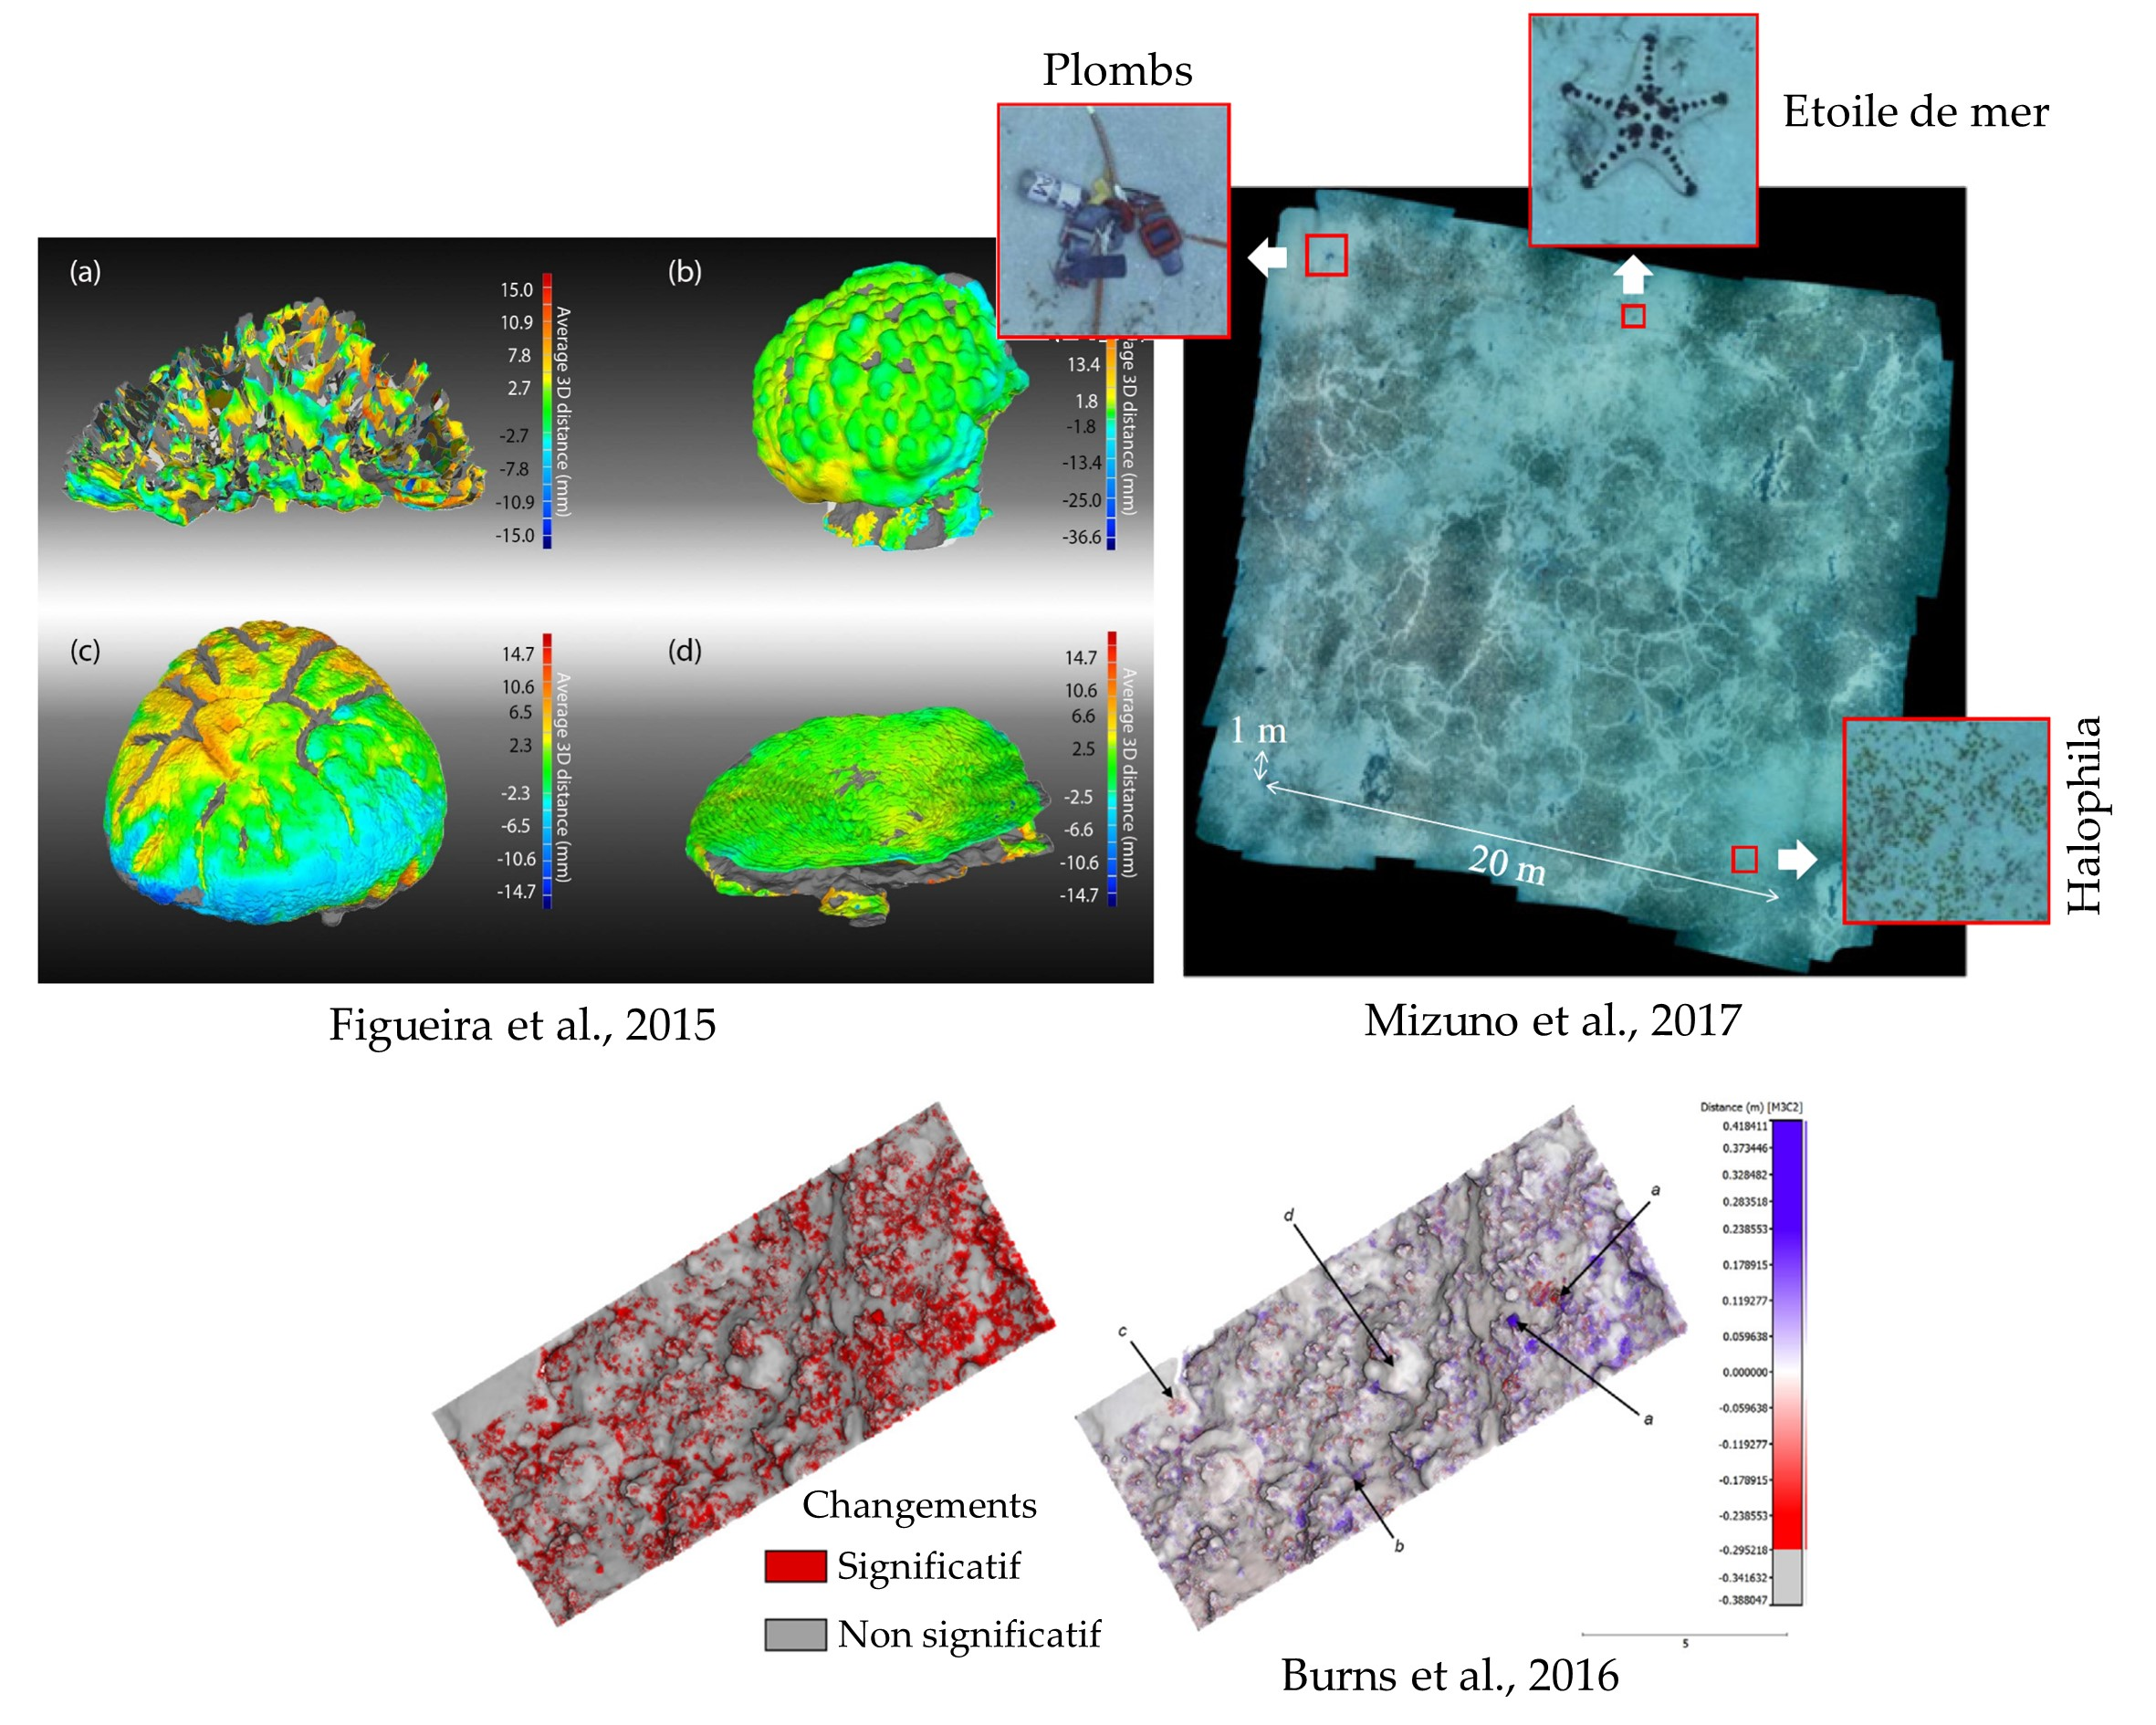
\includegraphics[width=\linewidth,keepaspectratio]{./2_methodes/PG_ecologie}
		\caption[Exemples d’applications photogrammétriques en écologie marine]{Exemples d’applications photogrammétriques en écologie marine. Haut gauche : mesures de précision de reconstructions de colonies de corail \citep{figueira_accuracy_2015} ; haut droit : cartographie d’herbiers et des zones de broutages de Dugong \citep{mizuno_simple_2017} ; bas : changements de morphologie d’un récif corallien à la suite d'une tempête tropicale \citep{burns_assessing_2016}.}
	\label{figure_methodo17}
\end{center}
\end{figure}